\documentclass[beamer=true]{standalone}
\usepackage{../../preamblesnotes}

%Information to be included in the title page:
\title{第二課}
\author{力和運動}
\institute{全年班}
\date{}

\begin{document}
\frame{\titlepage}

\begin{frame}{力的性質}
    \begin{itemize}
        \item 可分為接觸力和非接觸力。
              \begin{itemize}
                  \item 接觸力:包括張力、法向力、摩擦力、流體阻力;
                  \item 非接觸力:包括重量、電力、磁力。
              \end{itemize}
        \item 在國際單位制中,力的單位是牛頓,符號為\textbf{N}。

    \end{itemize}
\end{frame}

\begin{frame}{力的性質}
    \begin{itemize}
        \item 力是矢量,有量值和方向。向某方向作用的力,可用箭號來表示,箭號的方向和長度分別顯示力的方向和量值。
    \end{itemize}
\end{frame}

\begin{frame}{重量 (W) Weight (W)}
    \begin{itemize}
        \item 地球作用於物體的拉力。
        \item 方向指向地球的中心。
        \item W=mg, g = 重力加速度
    \end{itemize}
    \begin{columns}
        \column{.5\textwidth}
        \centering
        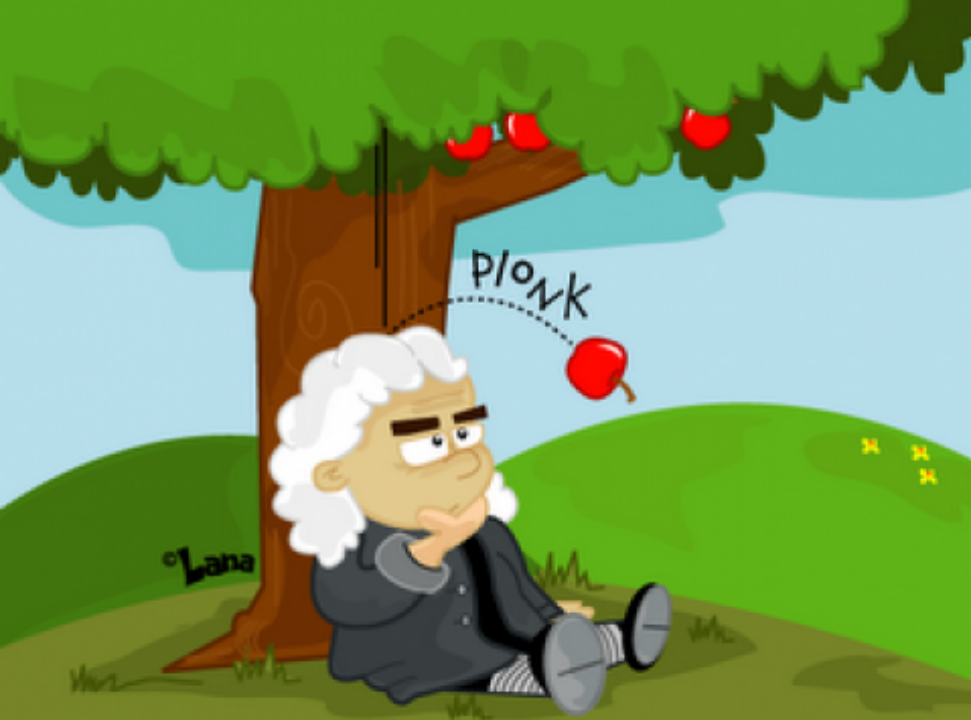
\includegraphics[width=\textwidth]{assets/47712628.png}
        \column{.5\textwidth}
        \begin{figure}[h!]
            \centering
            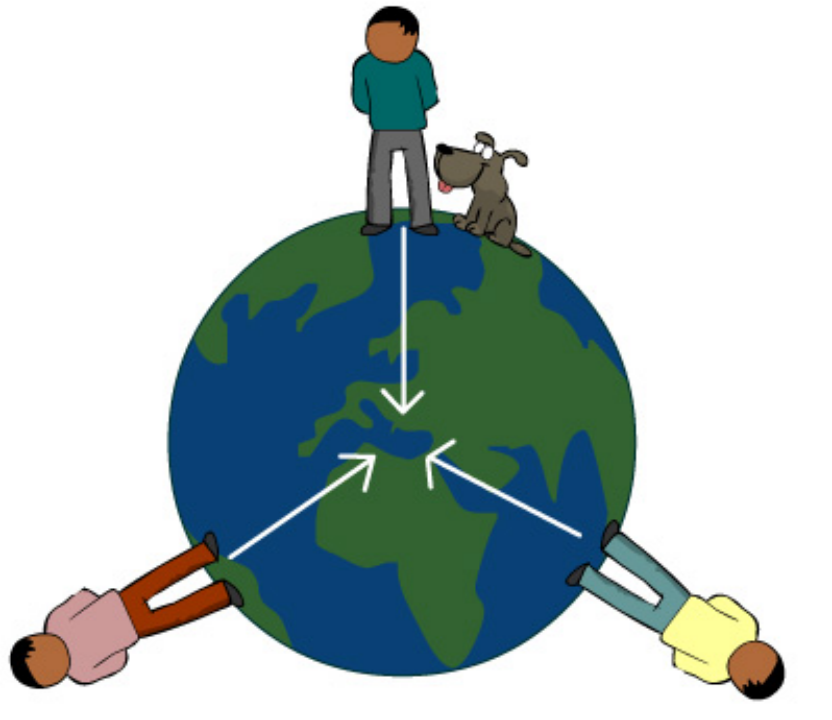
\includegraphics[width=\textwidth]{assets/97f12fb9.png}
        \end{figure}
    \end{columns}


\end{frame}


\begin{frame}{張力(T)}
    \begin{itemize}
        \item 繩子拉緊時產生的力。
        \item 在無質量的繩子裏,繩子每一點的張力量值都是相同的。
    \end{itemize}
    \begin{figure}[h!]
        \centering
        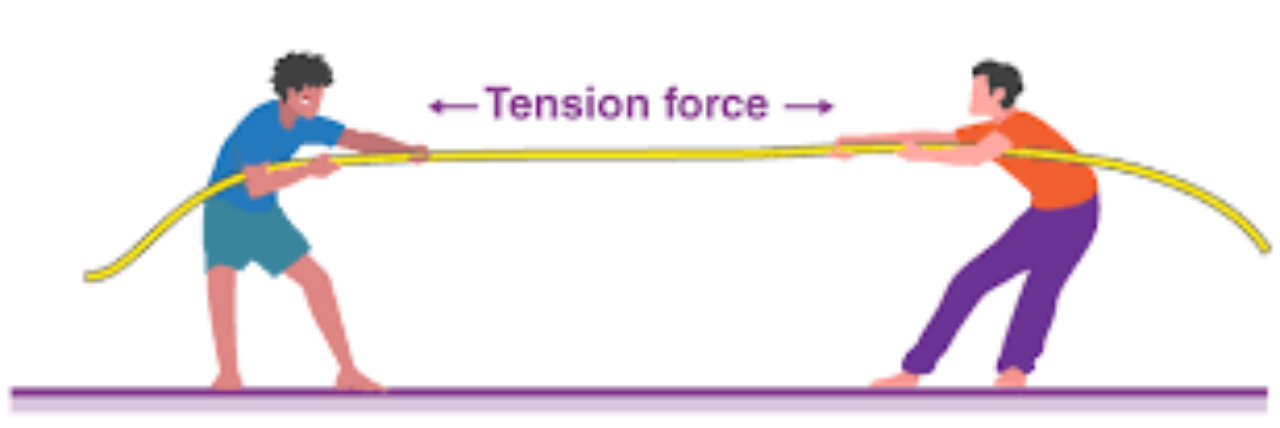
\includegraphics[width=0.66\textwidth]{assets/5673f702.png}
    \end{figure}
\end{frame}

\begin{frame}{法向力 (N 或 R) }
    \begin{itemize}
        \item 兩個物件的表面接觸所產生的力。
        \item 力和表面必定互相垂直。
    \end{itemize}
    \begin{figure}[h!]
        \centering
        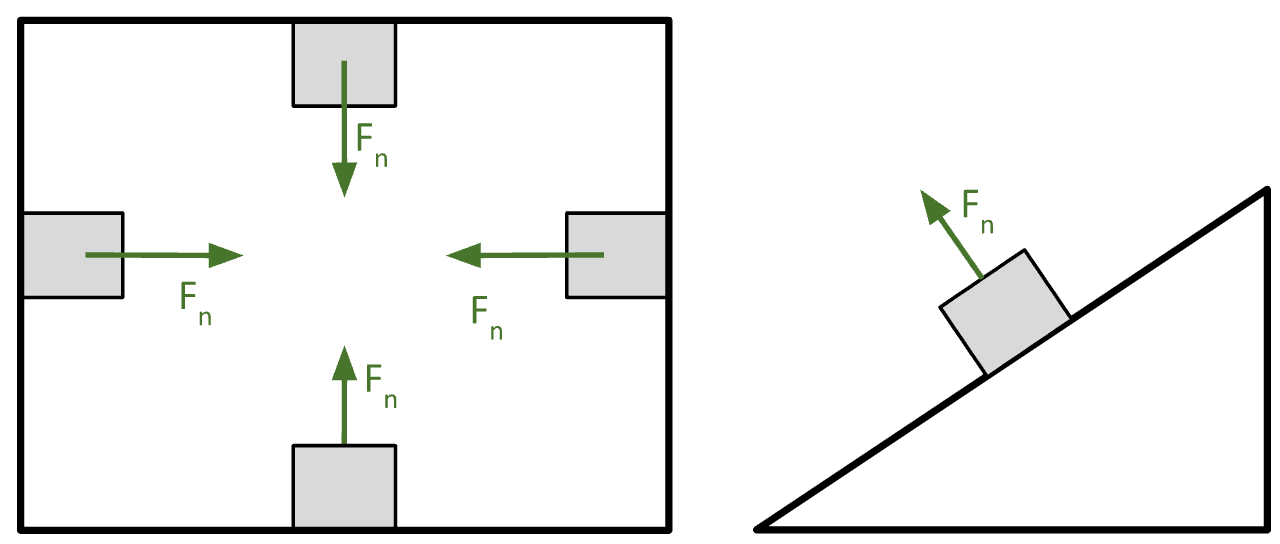
\includegraphics[width=.8\textwidth]{assets/77585bbc.png}
    \end{figure}
\end{frame}

\begin{frame}{阻力 (f) }
    \begin{itemize}
        \item 阻力是抗衡相對運動而產生的力。
        \item 例子:
              \begin{itemize}
                  \item 固體之間的摩擦力。
                  \item 空氣阻力。
                  \item 液體阻力。
                  \item 刹制力。
              \end{itemize}
    \end{itemize}

\end{frame}
\begin{frame}{摩擦力}

    \begin{itemize}
        \item 防止兩個接觸面發生相對運動所產生的力。
        \item 存在一個最大量值。
              \begin{itemize}
                  \item 摩擦力隨相對運動程度的增加而增加。沒有相對運動就沒有摩擦力。
                  \item 當摩擦力超過最大值時,摩擦力不會再增加。
              \end{itemize}
    \end{itemize}
    \begin{figure}[h!]
        \centering
        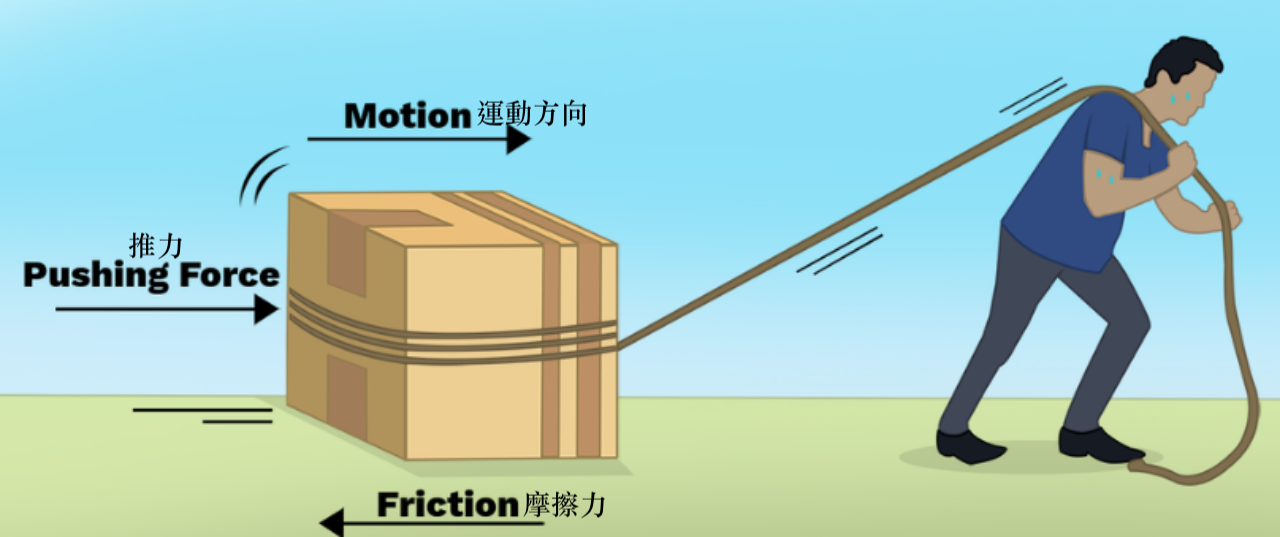
\includegraphics[width=.5\textwidth]{assets/48a9a34c.png}
    \end{figure}
\end{frame}

% \begin{frame}{降低摩擦力的方法}
% \begin{columns}
%     \column{.5\textwidth}
%     水平接觸面加上塑膠小珠\\add plastic bearings
% 接觸面加上油層\\add lubricating oil between contact surfaces
% 利用氣墊導航產生氣墊\\
%     \column{.5\textwidth}

% \end{columns}


% \end{frame}
% \begin{frame}{降低流線阻力的方法}
% 流線形設計\\streamline design
% \begin{columns}
%     \column{.5\textwidth}
%     \begin{figure}[h!]
% 	\centering
% 	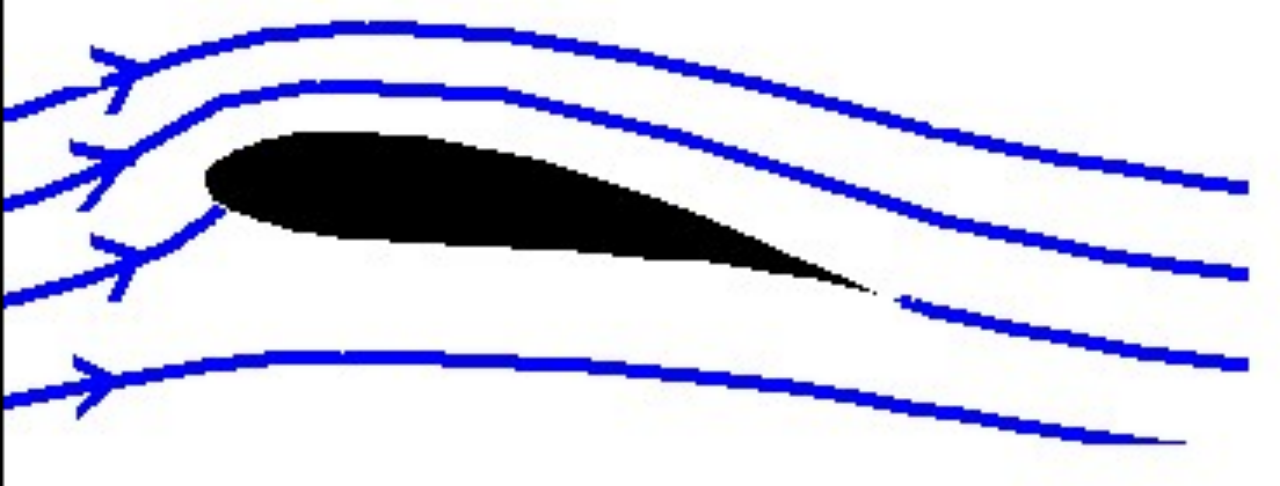
\includegraphics[width=.8\textwidth]{assets/710f9991.png}
% 	\end{figure}
%     \column{.5\textwidth}
%     \begin{figure}[h!]
% 	\centering
% 	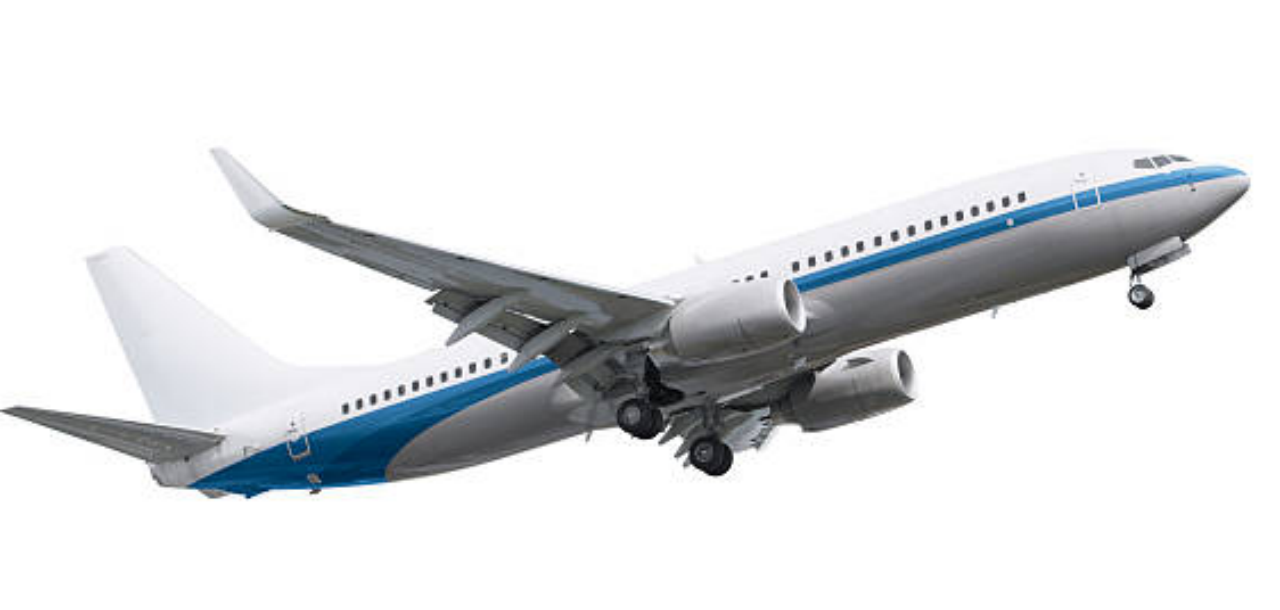
\includegraphics[width=.8\textwidth]{assets/4f685eca.png}
% 	\end{figure}
% \end{columns}
% \end{frame}

\begin{frame}{自由體圖/隔離體圖}
    \begin{itemize}
        \item 顯示所有作用於物體的力。\bigskip
    \end{itemize}
    \begin{figure}[h!]
        \centering
        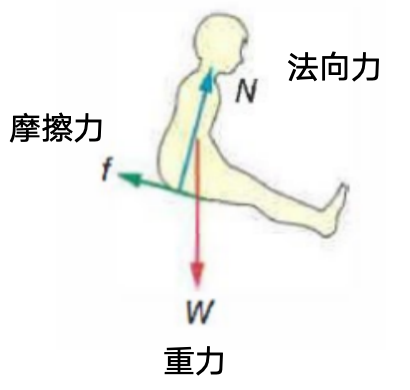
\includegraphics[width=0.5\textwidth]{assets/d2f67986.png}
    \end{figure}
\end{frame}



\begin{frame}{淨力/合力}
    \begin{itemize}
        \item 施加於物體的所有力的向量和。
    \end{itemize}\bigskip
    \begin{figure}[h!]
        \centering
        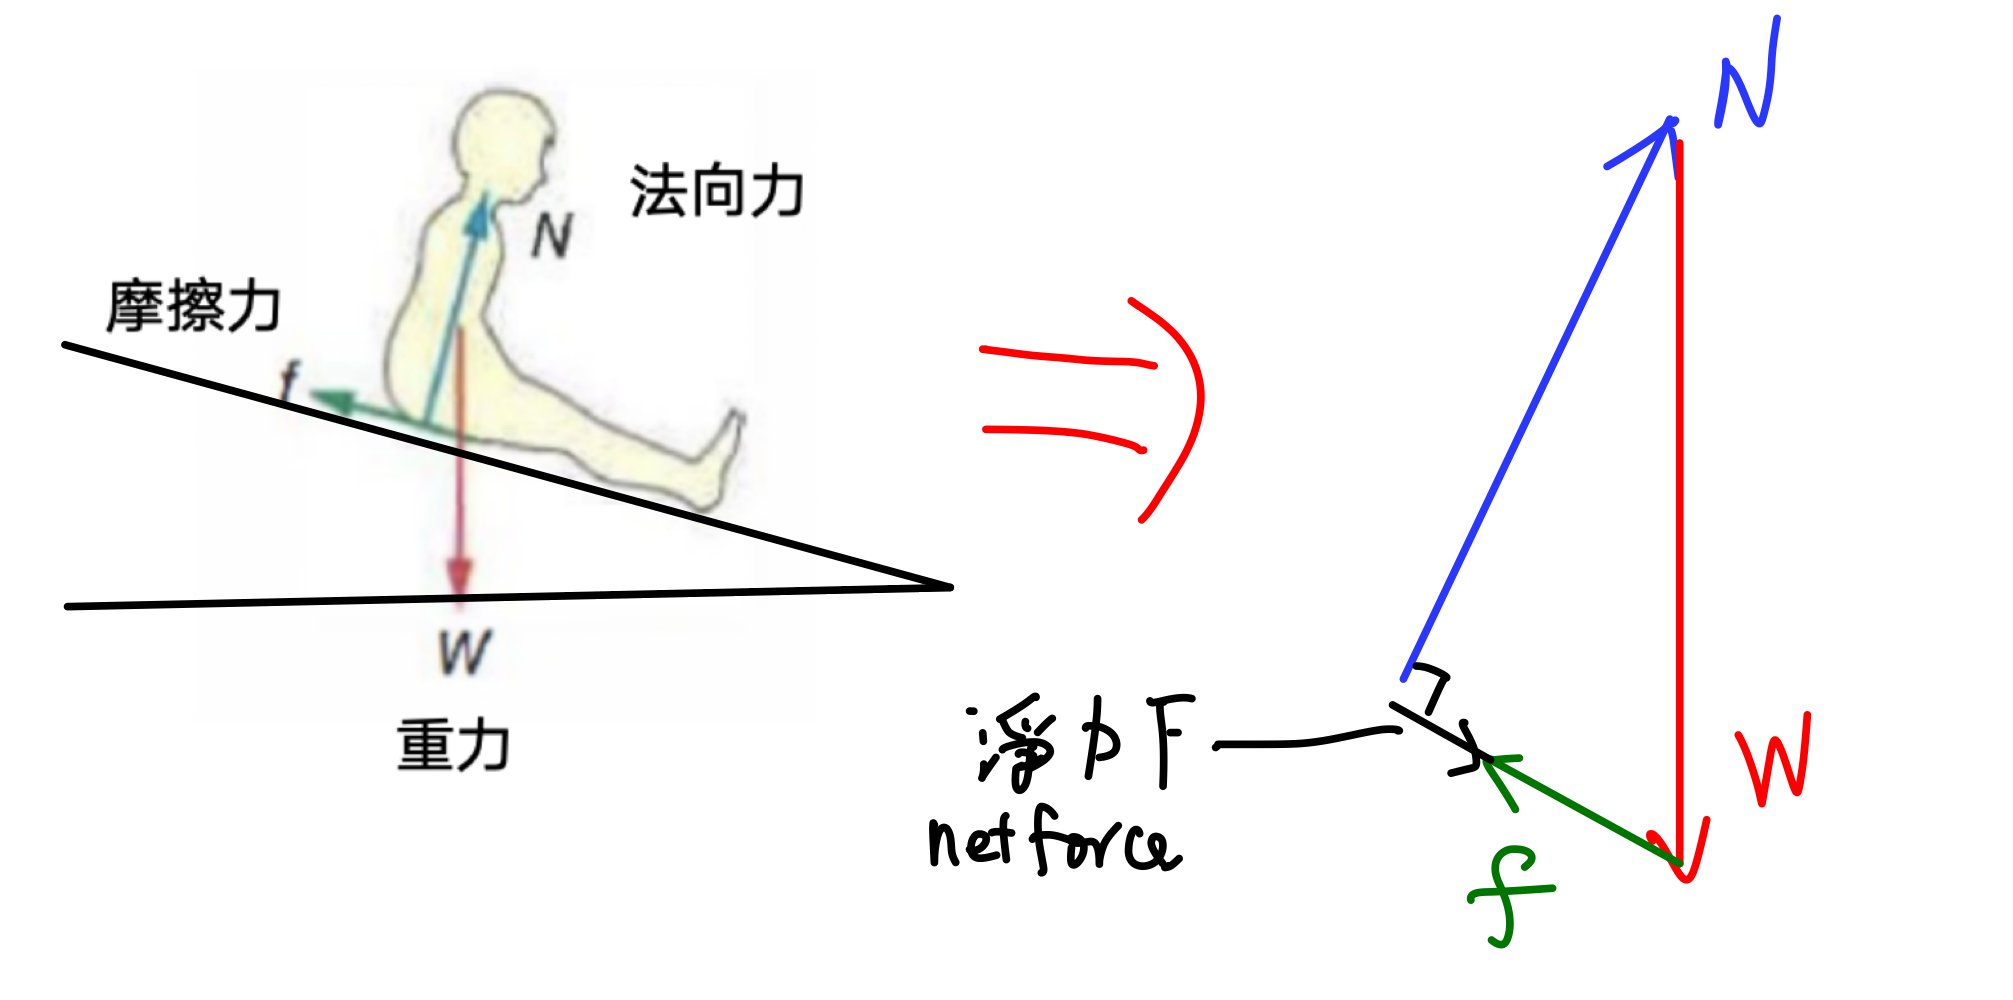
\includegraphics[width=.8\textwidth]{assets/96369bc9.png}
    \end{figure}
\end{frame}
\begin{frame}{淨力/合力}
    \begin{figure}[h!]
        \centering
        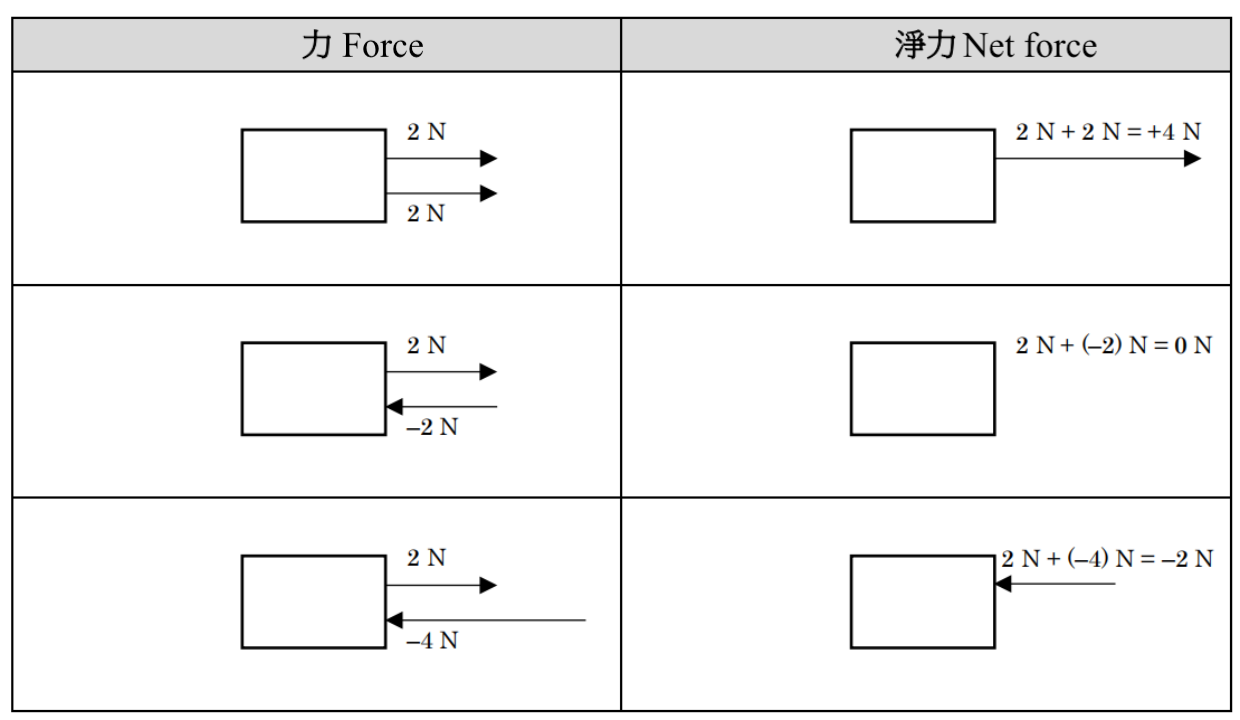
\includegraphics[width=\textwidth]{assets/5ffd7887.png}
    \end{figure}
\end{frame}
\begin{frame}{淨力/合力}
    \begin{figure}[h!]
        \centering
        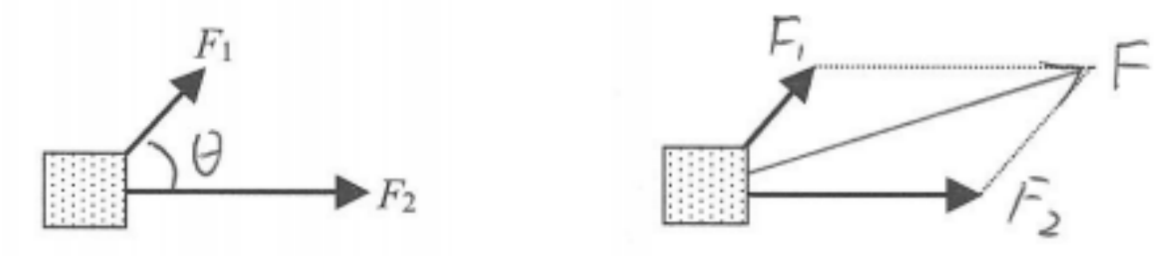
\includegraphics[width=.8\textwidth]{assets/61448695.png}
    \end{figure}
\end{frame}

\begin{frame}{力的拆解方法}
    \begin{figure}[h!]
        \centering
        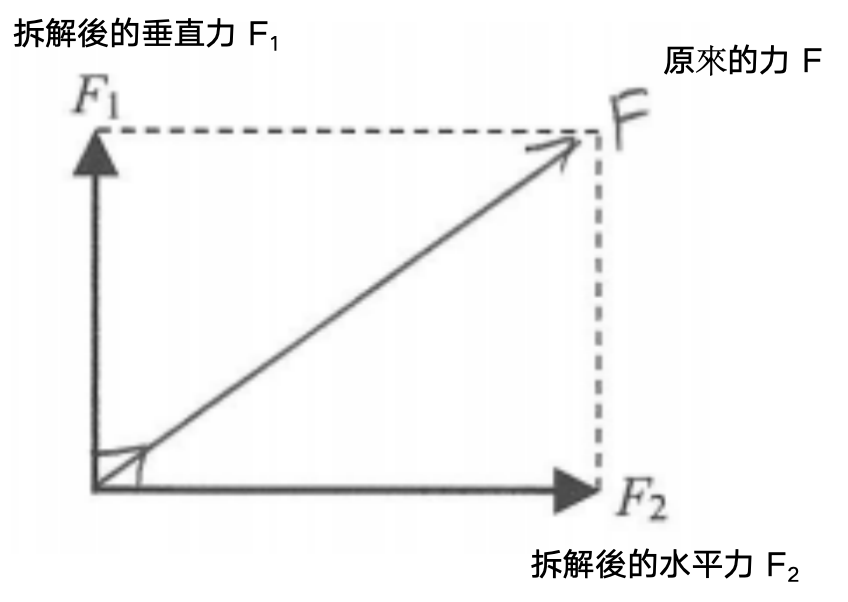
\includegraphics[width=0.66\textwidth]{assets/8695f254.png}
    \end{figure}
\end{frame}

\begin{eg}
    \begin{figure}[h!]
        \centering
        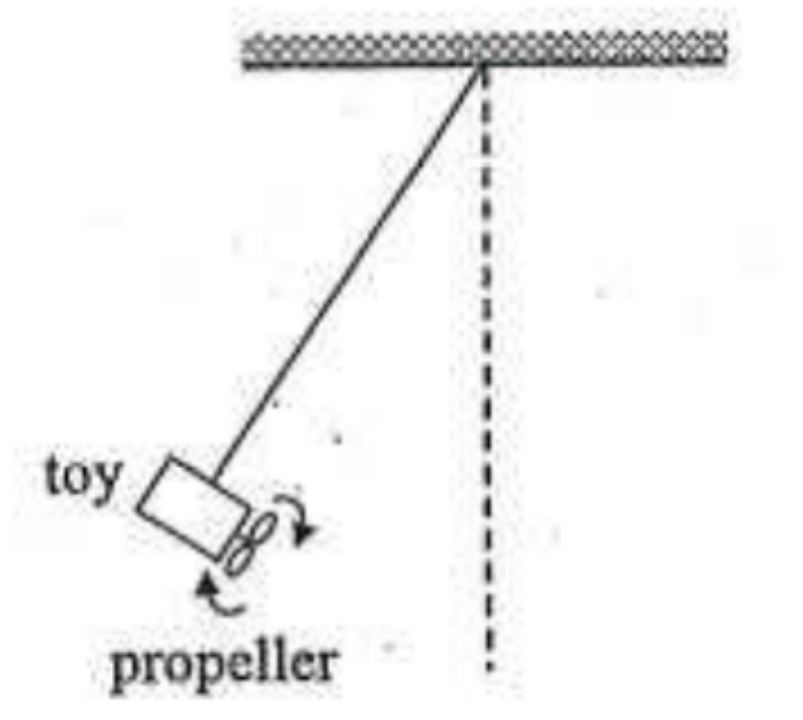
\includegraphics[width=0.35\textwidth]{assets/d7d1a80b.png}
    \end{figure}\bigskip\bigskip
    這個玩具裝了一個推進器和現在在靜止狀態。畫出這個玩具的自由體圖。
\end{eg}

\begin{frame}[t]{例題}
    如圖所示,兩個量使固定的力F$_1$及F$_2$作用於同一點,當F$_1$與F$_2$的夾角$\theta$由 \dg{0} 增加至 \dg{180},求合力的量值的變化。\\(a)增加(b)減少(c)先增加後減少(d)先減少後增加
    \begin{figure}[h!]
        \centering
        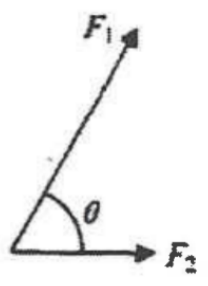
\includegraphics[width=.22\textwidth]{assets/11bd149b.png}
    \end{figure}
\end{frame}

\begin{frame}{有關力的定理}
    \begin{columns}
        \column{.4\textwidth}
        \begin{center}
            {\LARGE\textbf{牛頓力學定律}}
        \end{center}

        \column{.4\textwidth}
        \begin{figure}[h!]
            \centering
            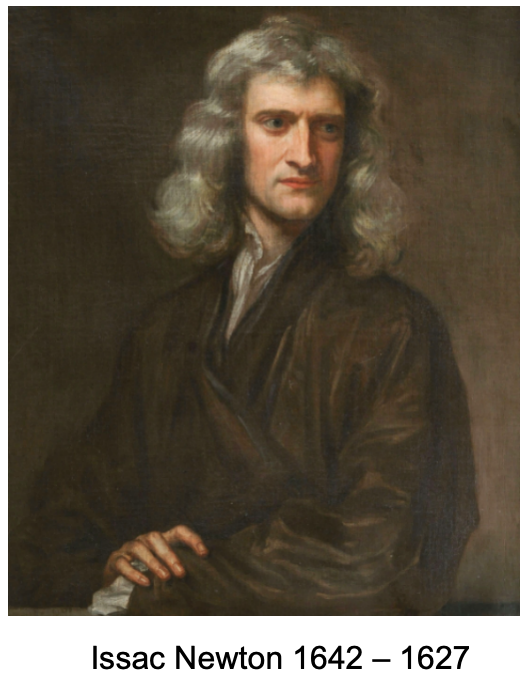
\includegraphics[width=.75\textwidth]{assets/57b990b1.png}
        \end{figure}

    \end{columns}
\end{frame}

\begin{frame}{牛頓第一定律和慣性}
    \begin{alertblock}
        {牛頓第一定律}
        除非受到淨力作用,否則所有物體都會保持靜止狀態或勻速直線運動狀態。
    \end{alertblock}
    \begin{exampleblock}
        {慣性}
        慣性是物體保持靜止或以均勻速度運動的趨勢。
    \end{exampleblock}
\end{frame}
\begin{frame}{牛頓第一定律和慣性}
    \begin{itemize}
        \item 慣性使物體繼續以勻速移動。\bigskip\bigskip
    \end{itemize}
    \begin{columns}
        \column{.33\textwidth}
        \begin{figure}[h!]
            \centering
            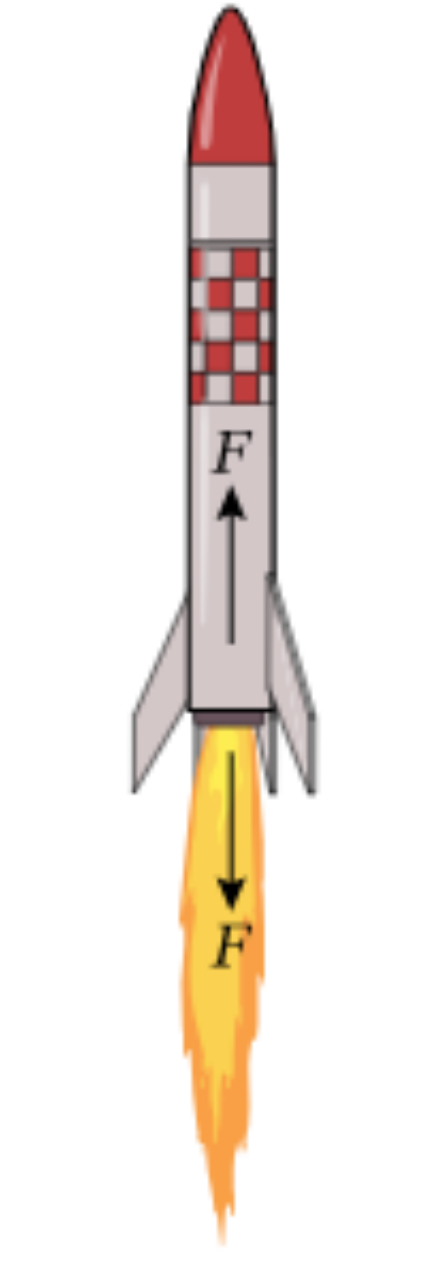
\includegraphics[width=0.4\textwidth]{assets/c32f5f7b.png}
        \end{figure}
        \column{.33\textwidth}
        \begin{figure}[h!]
            \centering
            
\includegraphics[width=.85\textwidth]{assets/b65bc2e1.png}
        \end{figure}
        \column{.33\textwidth}
        \begin{figure}[h!]
            \centering
            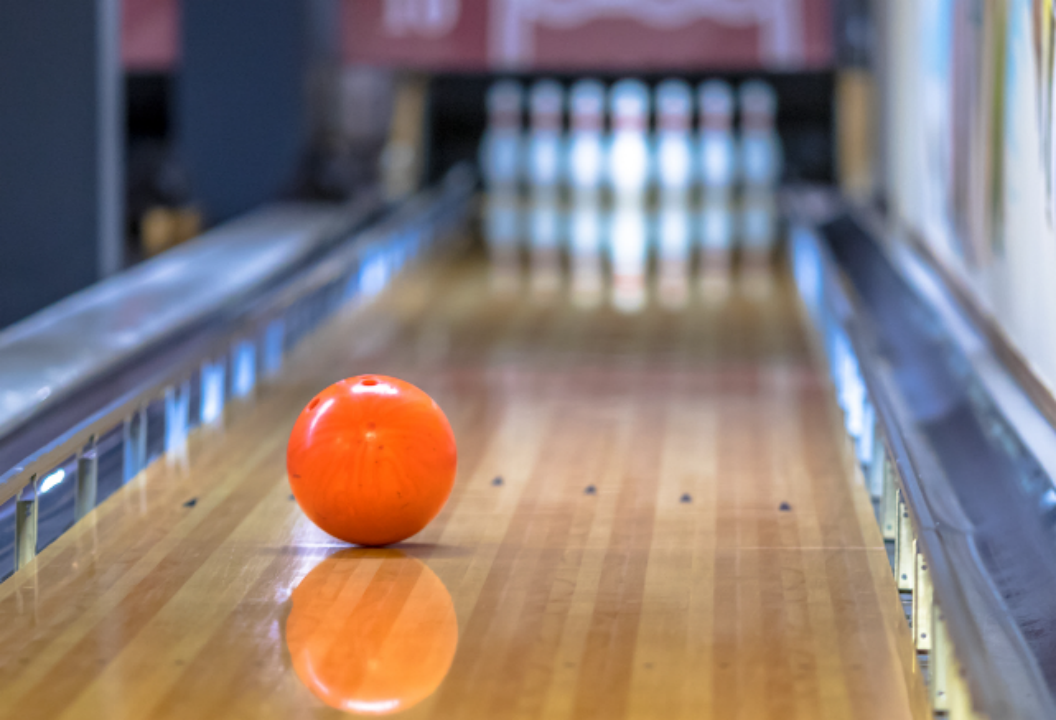
\includegraphics[width=.85\textwidth]{assets/888883a6.png}
        \end{figure}
    \end{columns}

\end{frame}

\begin{frame}{安全帶的應用}
    \begin{itemize}
        \item 當移動中的車子突然停車,因為慣性乘客會繼續前進。
        \item 安全帶可以防止乘客被拋出車外。
    \end{itemize}
    \begin{figure}[h!]
        \centering
        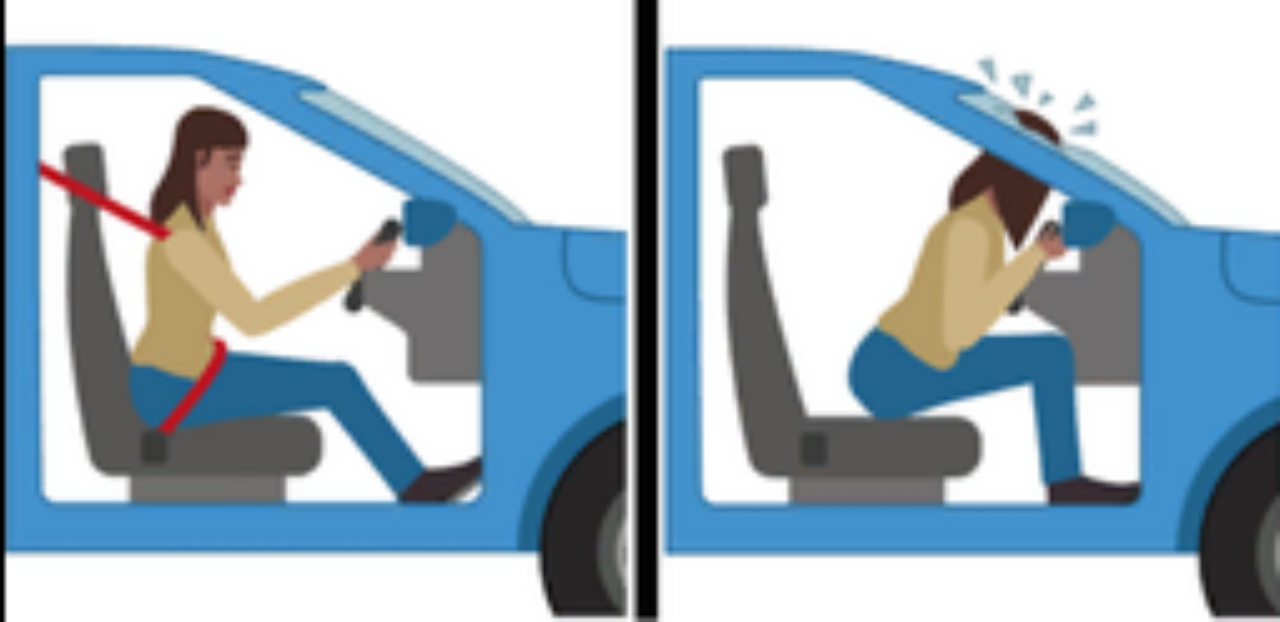
\includegraphics[width=.5\textwidth]{assets/88ea2a86.png}
    \end{figure}
\end{frame}

\begin{frame}{牛頓第一定律和慣性}
    \begin{itemize}
        \item 慣性使物體繼續靜止。
    \end{itemize}
    \begin{figure}[h!]
        \centering
        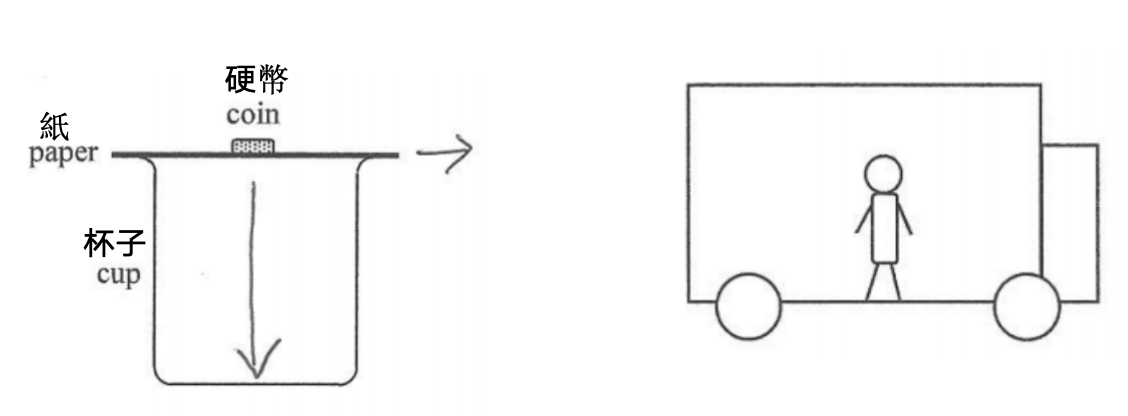
\includegraphics[width=0.85\textwidth]{assets/d5349655.png}
    \end{figure}
\end{frame}

\begin{frame}{牛頓第一定律和慣性 }
    \begin{itemize}
        \item 慣性使物體繼續靜止。
    \end{itemize}
    \begin{columns}
        \column{.6\textwidth}
        \begin{itemize}
            \item 慢拉線$\Rightarrow$上面先斷
                  \begin{itemize}
                      \item 上面部分承受更大的張力。
                  \end{itemize}
            \item 快拉線 $\Rightarrow$ 下面先斷
                  \begin{itemize}
                      \item 物件傾向保持靜止狀態。
                  \end{itemize}
        \end{itemize}
        \column{.4\textwidth}
        \begin{figure}[h!]
            \centering
            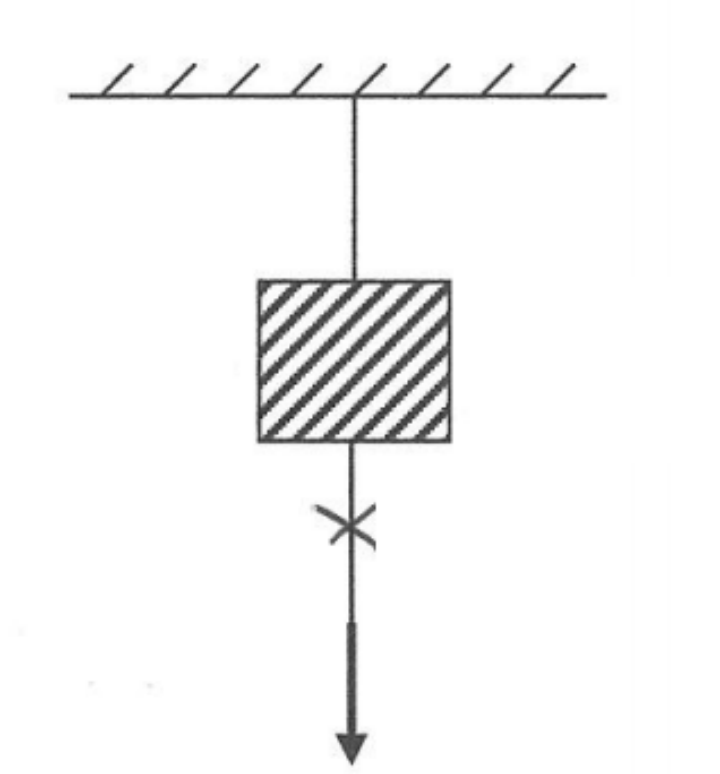
\includegraphics[width=.8\textwidth]{assets/842a74ec.png}
        \end{figure}
    \end{columns}
\end{frame}



\begin{frame}{牛頓第二定律}
    \begin{alertblock}
        {牛頓第二定律}
        \begin{equation}
            \vec{F}=m\vec{a}
        \end{equation}
    \end{alertblock}
    \begin{itemize}

        \item 物件受到的淨力 F 與物件的質量 m 及加速度 a 成正比,且淨力和加速度方向相同,且量值滿足 $F=m a$ 。
        \item 淨力、質量和加速度分別採用S.I.單位牛頓(N)、千克(kg)和米每平方秒(\acc{})。
    \end{itemize}
\end{frame}

\begin{eg}
    一塊起始靜止的方塊放在光滑的桌子上,被一個水平的恆定力 F 推動。利用牛頓運動定律,解釋為什麼這個方塊應該開始移動。
    \begin{itemize}
        \item [解] 施加在方塊上垂直方向的合力(重力和法向反作用力)是平衡的。水平方向有非零的淨力F作用於方塊上。\\根據牛頓第二定律,方塊應該會有與力同方向的加速度。
    \end{itemize}
\end{eg}

\begin{eg}
    一個球質量為 4 kg,它被輕推了一下後,以速率\vel{2}運動。10 s後,它停了下來。
    \begin{itemize}
        \item[(a)] 求球與地面間的摩擦力。
    \end{itemize}
\end{eg}
\begin{eg}
    一個球質量為 4 kg,它被輕推了一下後,以速率\vel{2}運動。10 s後,它停了下來。
    \begin{itemize}
        \item[(b)] 如果摩擦力減半而其他因素不變,球移動的距離是多少?
    \end{itemize}
\end{eg}
\begin{eg}
    一個球質量為 4 kg,它被輕推了一下後,以速率\vel{2}運動。10 s後,它停了下來。
    \begin{itemize}
        \item[(c)] 如果摩擦力加倍而其他因素不變,球移動的時間是?
    \end{itemize}
\end{eg}


\begin{eg}
    一個男孩的質量是 30 kg。他以\vel{5}垂直到達水面且他最深下降至 \qty{2}{m}。求水對男孩施力的量值。
\end{eg}

\begin{frame}{拆力相關題目}
    \begin{itemize}
        \item 把力分解成水平和垂直方向。
              \begin{itemize}
                  \item 然後把該方向的所有力放一邊,ma放另一邊。
                  \item 如果是靜止/勻速,一邊方向的所有力=另一邊方向的所有力。
              \end{itemize}
        \item 斜坡問題:
              \begin{itemize}
                  \item 把力分解成沿鈄坡,和垂直於斜坡。
              \end{itemize}
    \end{itemize}
\end{frame}

\begin{frame}[t]{例題}
    \begin{figure}[h!]
        \centering
        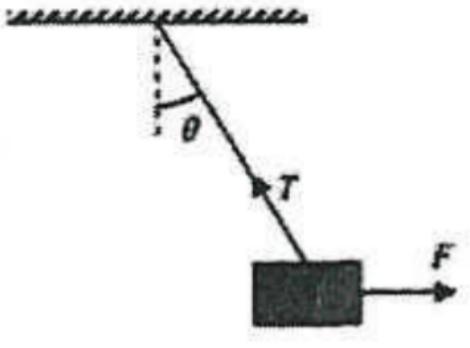
\includegraphics[width=0.3\textwidth]{assets/0b66fd6a.png}
    \end{figure}
    % 上圖中,一方塊以一繩子掛於天花板,水平力F作用在該方塊上。於平衡狀態時,繩子和豎直成角$\theta$,而繩子的張力為T。以F和$\theta$表示該方塊的重量。\\In the given diagram, a block is suspended from the ceiling by a rope, and a horizontal force F is applied to the block. In the equilibrium state, the rope forms an angle $\theta$ with the vertical, and the tension in the rope is T. Find the weight of the block in terms of F and $\theta$. 
    以F和$\theta$表示方塊的重量。
\end{frame}

\begin{eg}
    揚浩將手推車推上斜坡。他施於手推車的力平行於斜坡,量值為 200 N。斜坡與水平線的夾角為 \oc{10}。手推車連貨物的質量為 50 kg,斜坡施於手推車的摩擦力為 80 N。

    \begin{itemize}
        \item[(a)] 斜坡施於手推車的法向力,量值是多少?
    \end{itemize}

\end{eg}
\begin{eg}
    揚浩將手推車推上斜坡。他施於手推車的力平行於斜坡,量值為 200 N。斜坡與水平線的夾角為 \dg{10}。手推車連貨物的質量為 50 kg,斜坡施於手推車的摩擦力為 \qty{80}{N}。
    \begin{itemize}
        \item[(b)] 求手推車的加速度量值。
    \end{itemize}
\end{eg}

\begin{frame}{滑輪問題}
    \begin{itemize}
        \item \textbf{輕質不可延伸}的繩子:繩子上每一個點的張力皆為\textbf{零}。
        \item \textbf{光滑}滑輪:滑輪兩邊的張力量值\textbf{相等}。
    \end{itemize}
    \begin{figure}[h!]
        \centering
        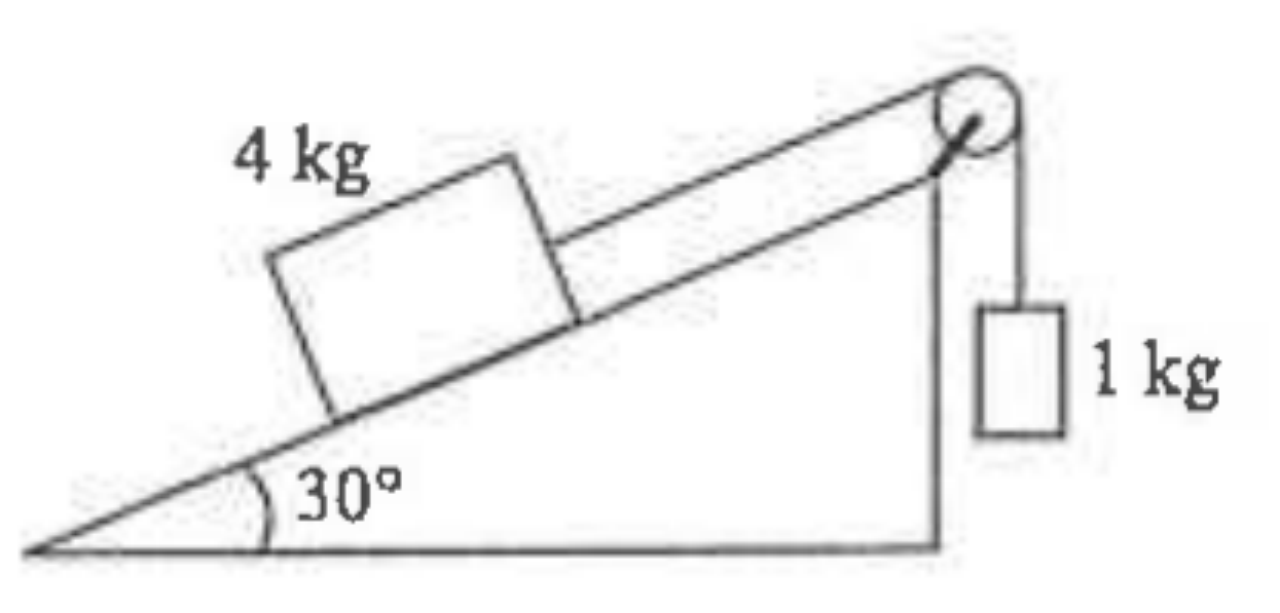
\includegraphics[width=0.4\textwidth]{assets/54dc796f.png}
    \end{figure}
\end{frame}


\begin{eg}
    \begin{figure}[h!]
        \centering
        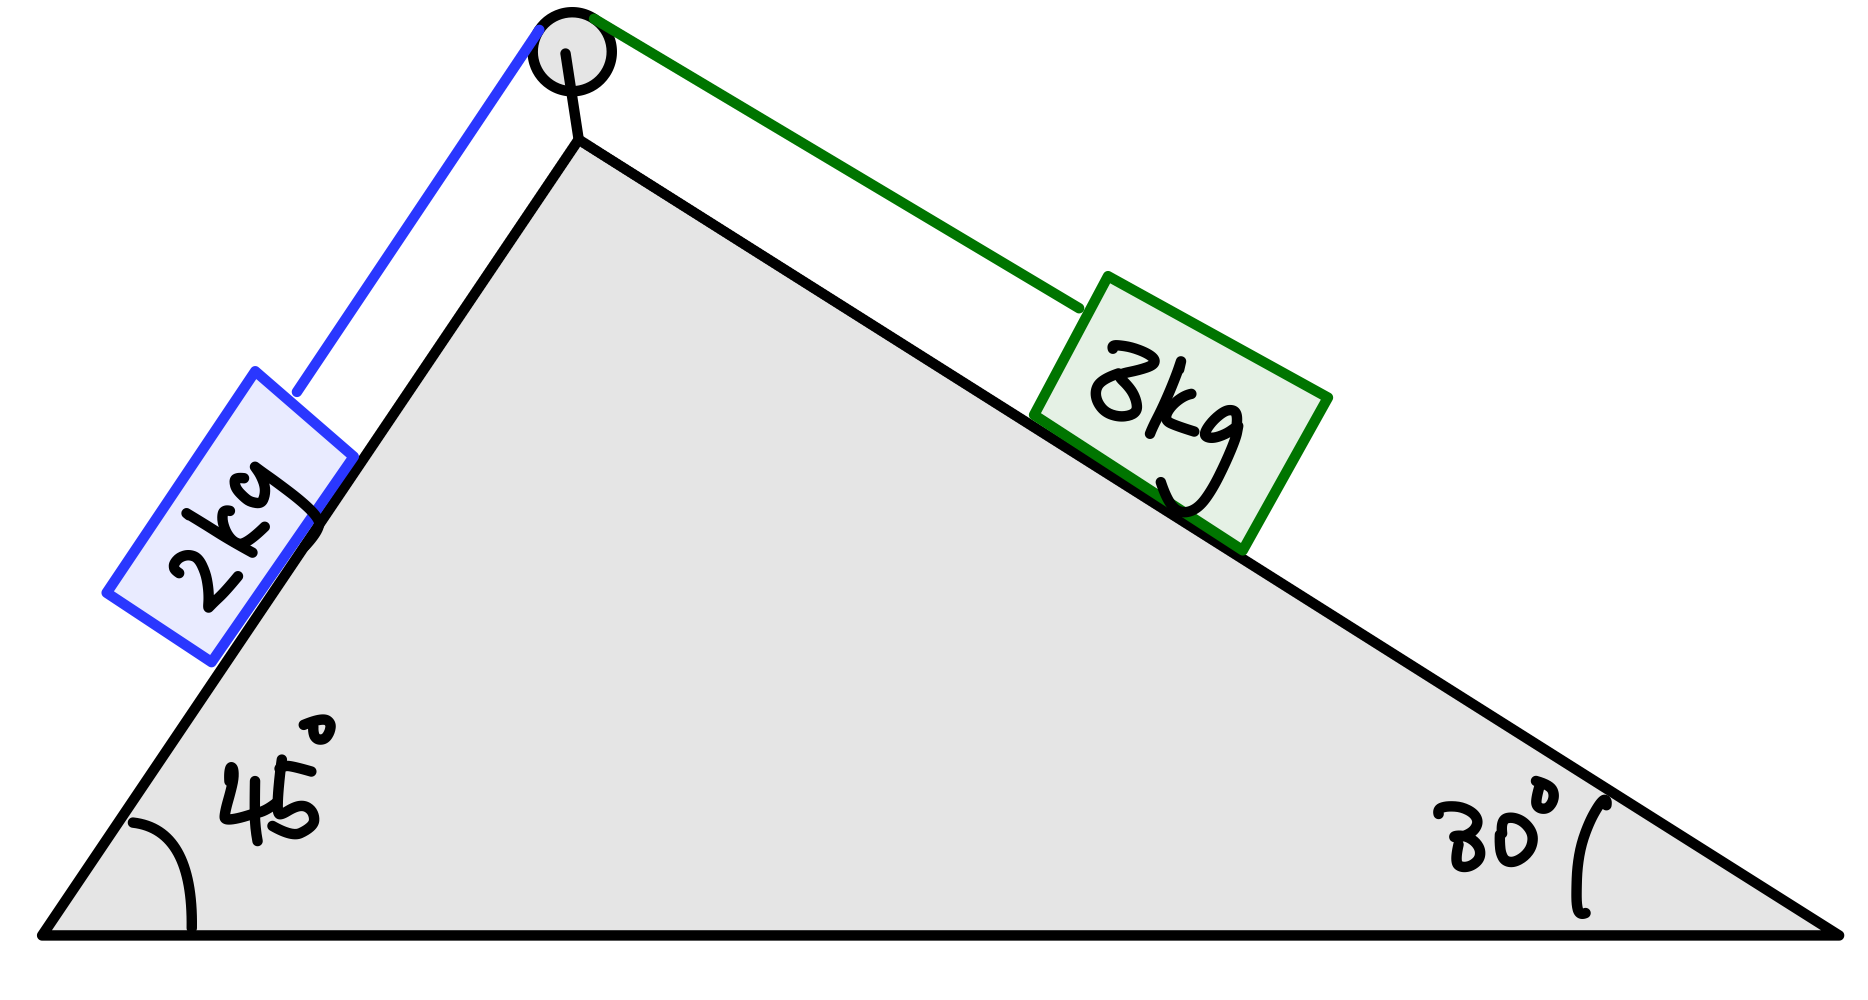
\includegraphics[width=0.4\textwidth]{assets/a078f185.png}
    \end{figure}
    所有表面光滑,取重力加速度 g = \acc{9.81}。求繩子的張力。
\end{eg}



\begin{eg}
    \begin{figure}[h!]
        \centering
        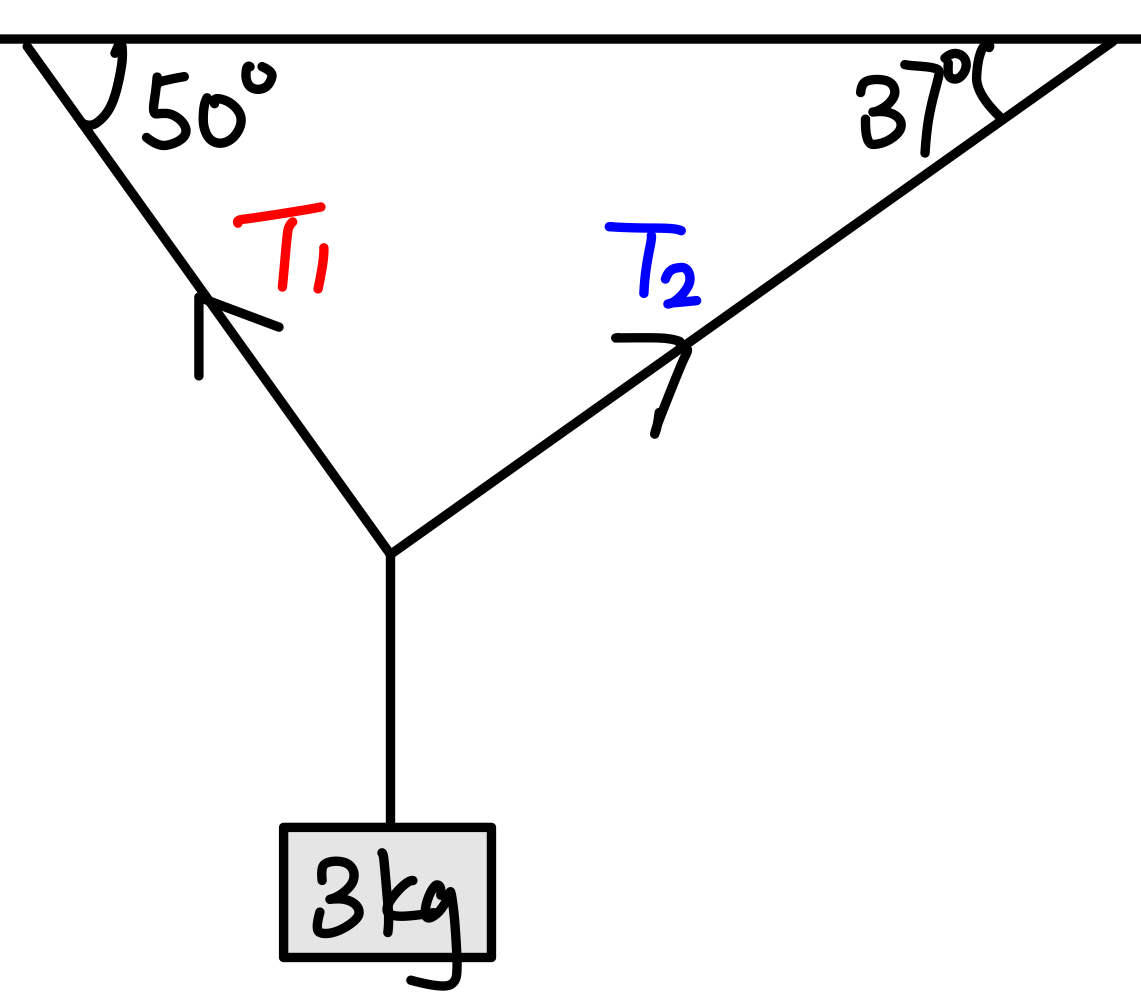
\includegraphics[width=.3\textwidth]{assets/ce5681cb.png}
    \end{figure}
    取重力加速度 g = \acc{9.81}。求繩子的張力T$_1$和T$_2$。
\end{eg}

\begin{frame}{升降機問題}
    假設這人有50kg, 取$g$ = \acc{10}

    \begin{columns}
        \column{.65\textwidth}
        \begin{itemize}
            \setlength{\itemsep}{10pt}
            \item 電梯是均速率
            \item 電梯以\acc{1}向上加速\\$\Rightarrow N-mg=ma$\\$\Rightarrow N=550$N\\感覺重了。

            \item 電梯以\acc{1}向下加速 \\$\Rightarrow mg-N=ma$\\$\Rightarrow N=450$N\\感覺輕了。
                  % \item 電梯以$>$ \acc{g} 向下加速\\the elevator accelerates downwards with $>$ \acc{g}: N=0
                  % \item N=表觀重量apparant weight
        \end{itemize}
        \column{.3\textwidth}
        \begin{figure}[h!]
            \centering
            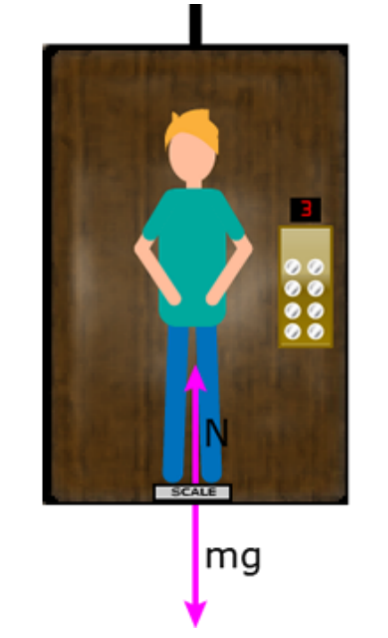
\includegraphics[width=\textwidth]{assets/6596ff5b.png}
        \end{figure}
    \end{columns}
\end{frame}
\begin{frame}{升降機問題}
    假設這人有50kg, 取$g$ = \acc{10}

    \begin{columns}
        \column{.65\textwidth}
        \begin{itemize}
            \setlength{\itemsep}{15pt}

            \item 電梯以 $>$ $g$\acc{} 向下加速 \\$\Rightarrow N=0$
            \item $N=$ \textbf{表觀重量}
        \end{itemize}
        \column{.3\textwidth}
        \begin{figure}[h!]
            \centering
            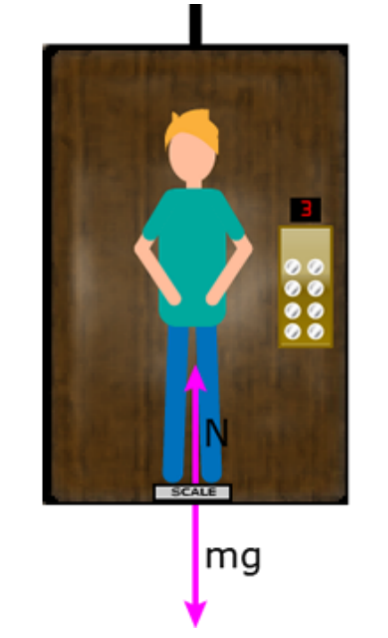
\includegraphics[width=\textwidth]{assets/6596ff5b.png}
        \end{figure}
    \end{columns}
\end{frame}

\begin{frame}{流體阻力}
    \begin{exampleblock}
        {流體阻力}
        \begin{equation}
            f=k \;\rho\; v^2\; A
        \end{equation}
    \end{exampleblock}
    \begin{itemize}
        \item k = 常數, $\rho$ = 流體密度, $v$ = 速率, \\$A$ = 橫截面面積
              % \item 跳傘員不開跳傘降落時,\\When skydiver falls without parachute,
              % \begin{itemize}
              %     \item 加速度向下 accelerates downwards: $W-f=ma$
              %     \item v逐漸增加gradually increases $\Rightarrow$ f 逐漸增加gradually increases
              % \end{itemize}

    \end{itemize}
    \bigskip
    \begin{figure}[h!]
        \centering
        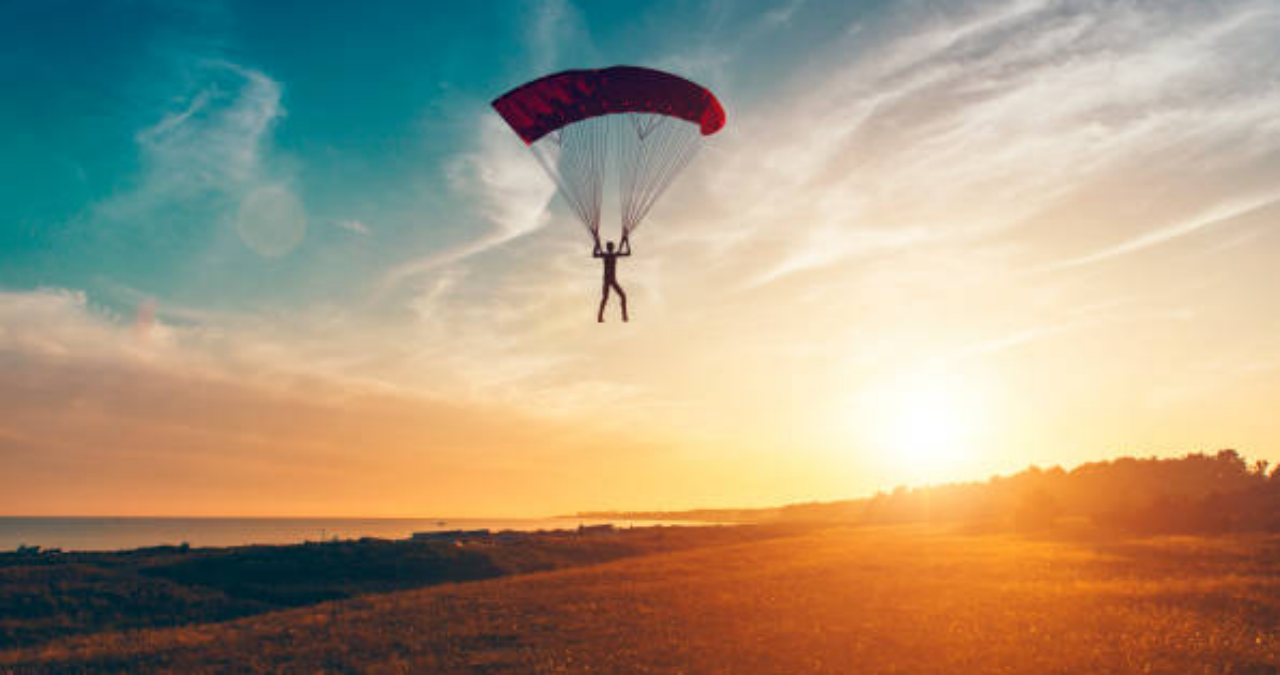
\includegraphics[width=.4\textwidth]{assets/31e14542.png}
    \end{figure}
\end{frame}
\begin{frame}{流體阻力}
    \begin{itemize}
        \item 跳傘員不開跳傘降落時,
              \begin{itemize}
                  \item 加速度向下  $W-f=ma$
                  \item v逐漸增加 $\Rightarrow$ f 逐漸增加gradually
                  \item 直到f 完全扺消 W,淨力變成零:  $W-f=0$
                  \item 加速度為零,以\textbf{恆定}的\textbf{終端速率}繼續落下。
              \end{itemize}
    \end{itemize}
    \begin{figure}[h!]
        \centering
        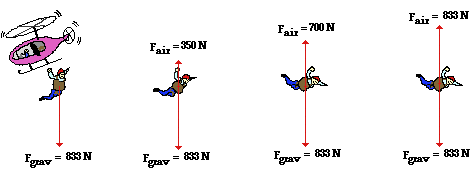
\includegraphics[width=.7\textwidth]{assets/e052106e.png}
    \end{figure}
\end{frame}
\begin{frame}{流體阻力}
    \begin{itemize}
        \item 當在終端速率的跳傘員突然打開跳傘,
              \begin{itemize}
                  \item 橫截面面積突然增加,f突然增加。
                  \item 淨力向上,跳傘員向下減速。
                  \item f持續下降至淨力為零。
                  \item 以\textbf{更低}的終端速率落下。
              \end{itemize}
    \end{itemize}

    \begin{figure}[h!]
        \centering
        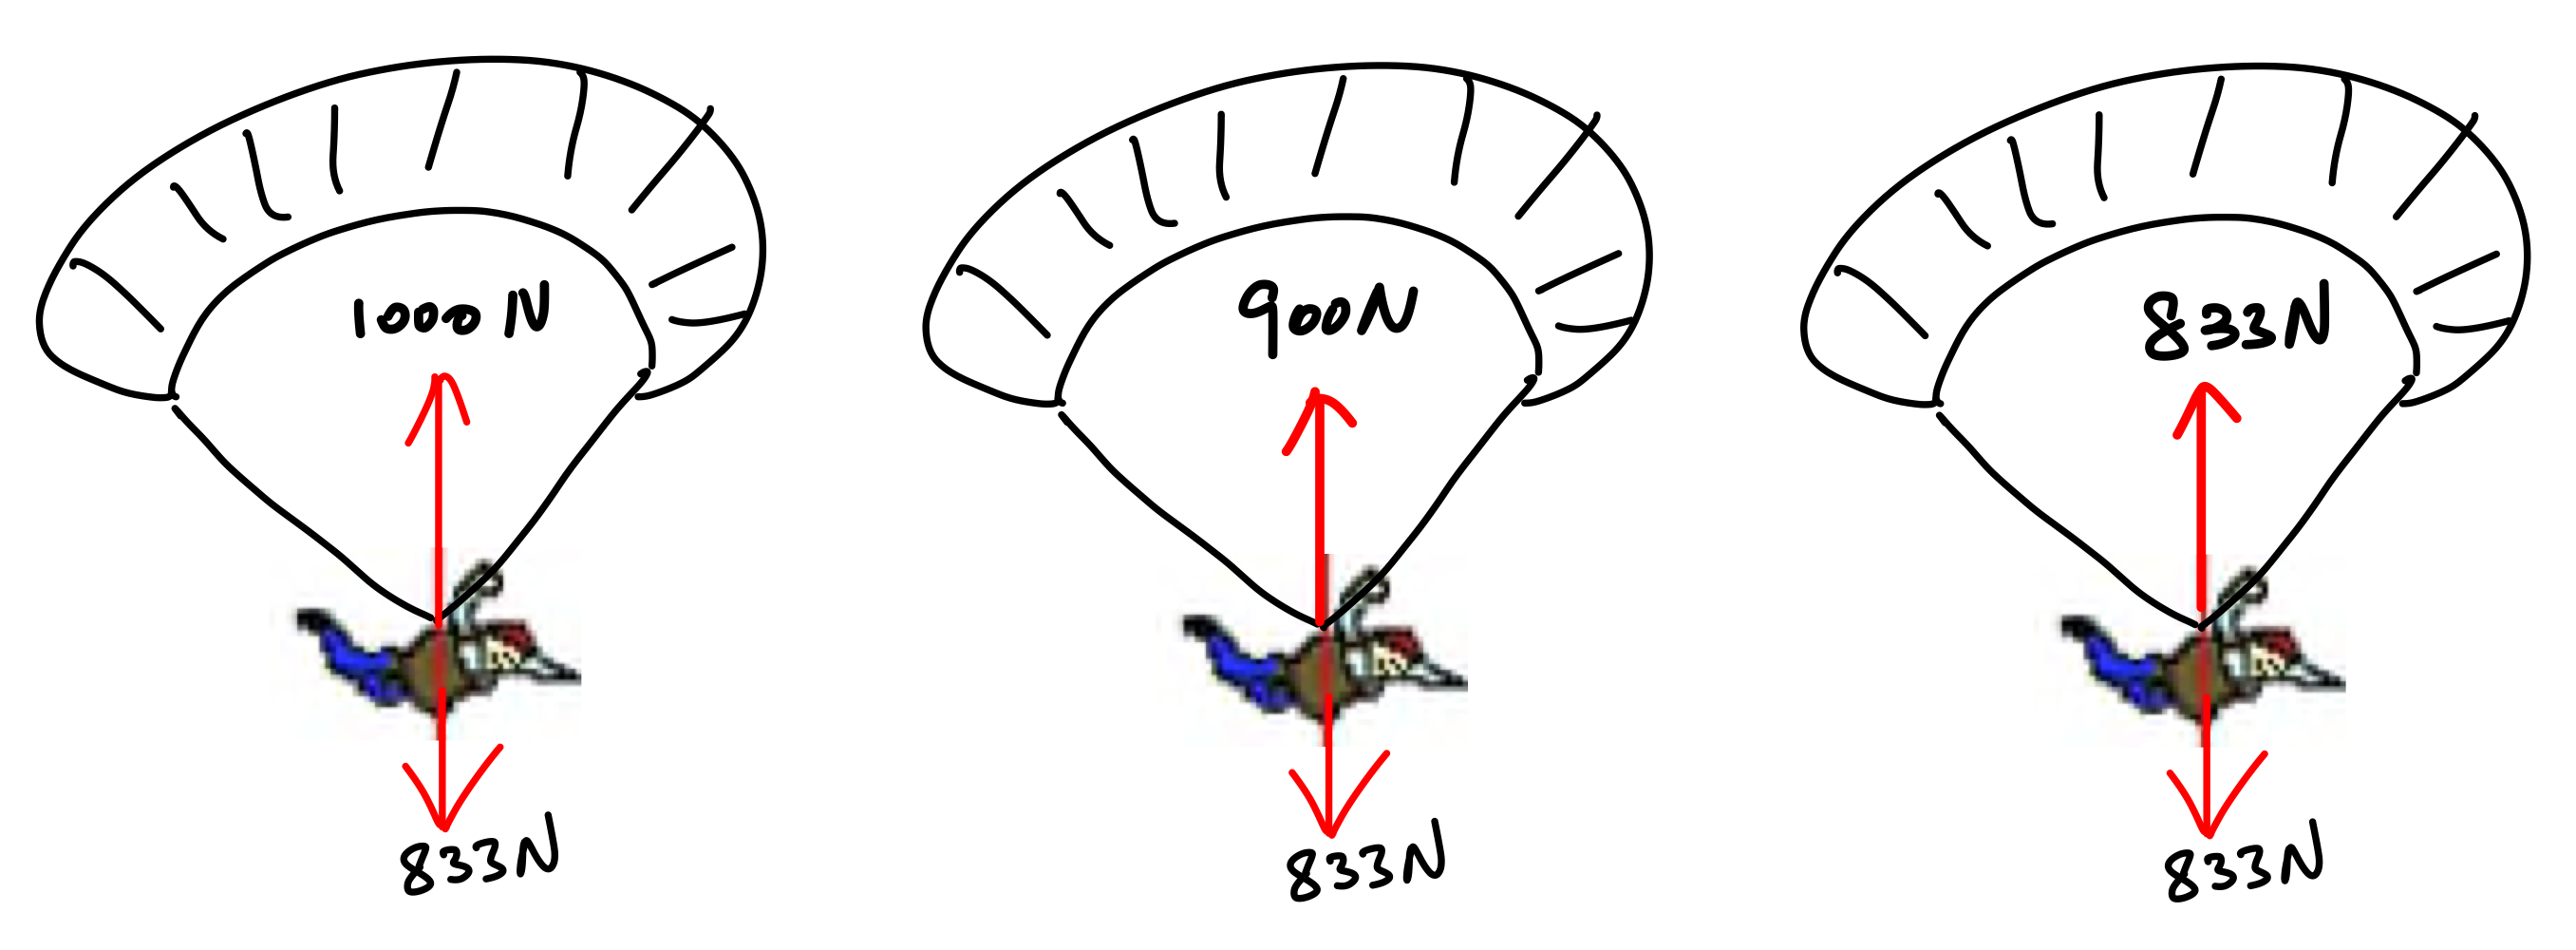
\includegraphics[width=.55\textwidth]{assets/bacb418f.png}
    \end{figure}

\end{frame}

\begin{frame}{流體阻力}
    \begin{figure}[h!]
        \centering
        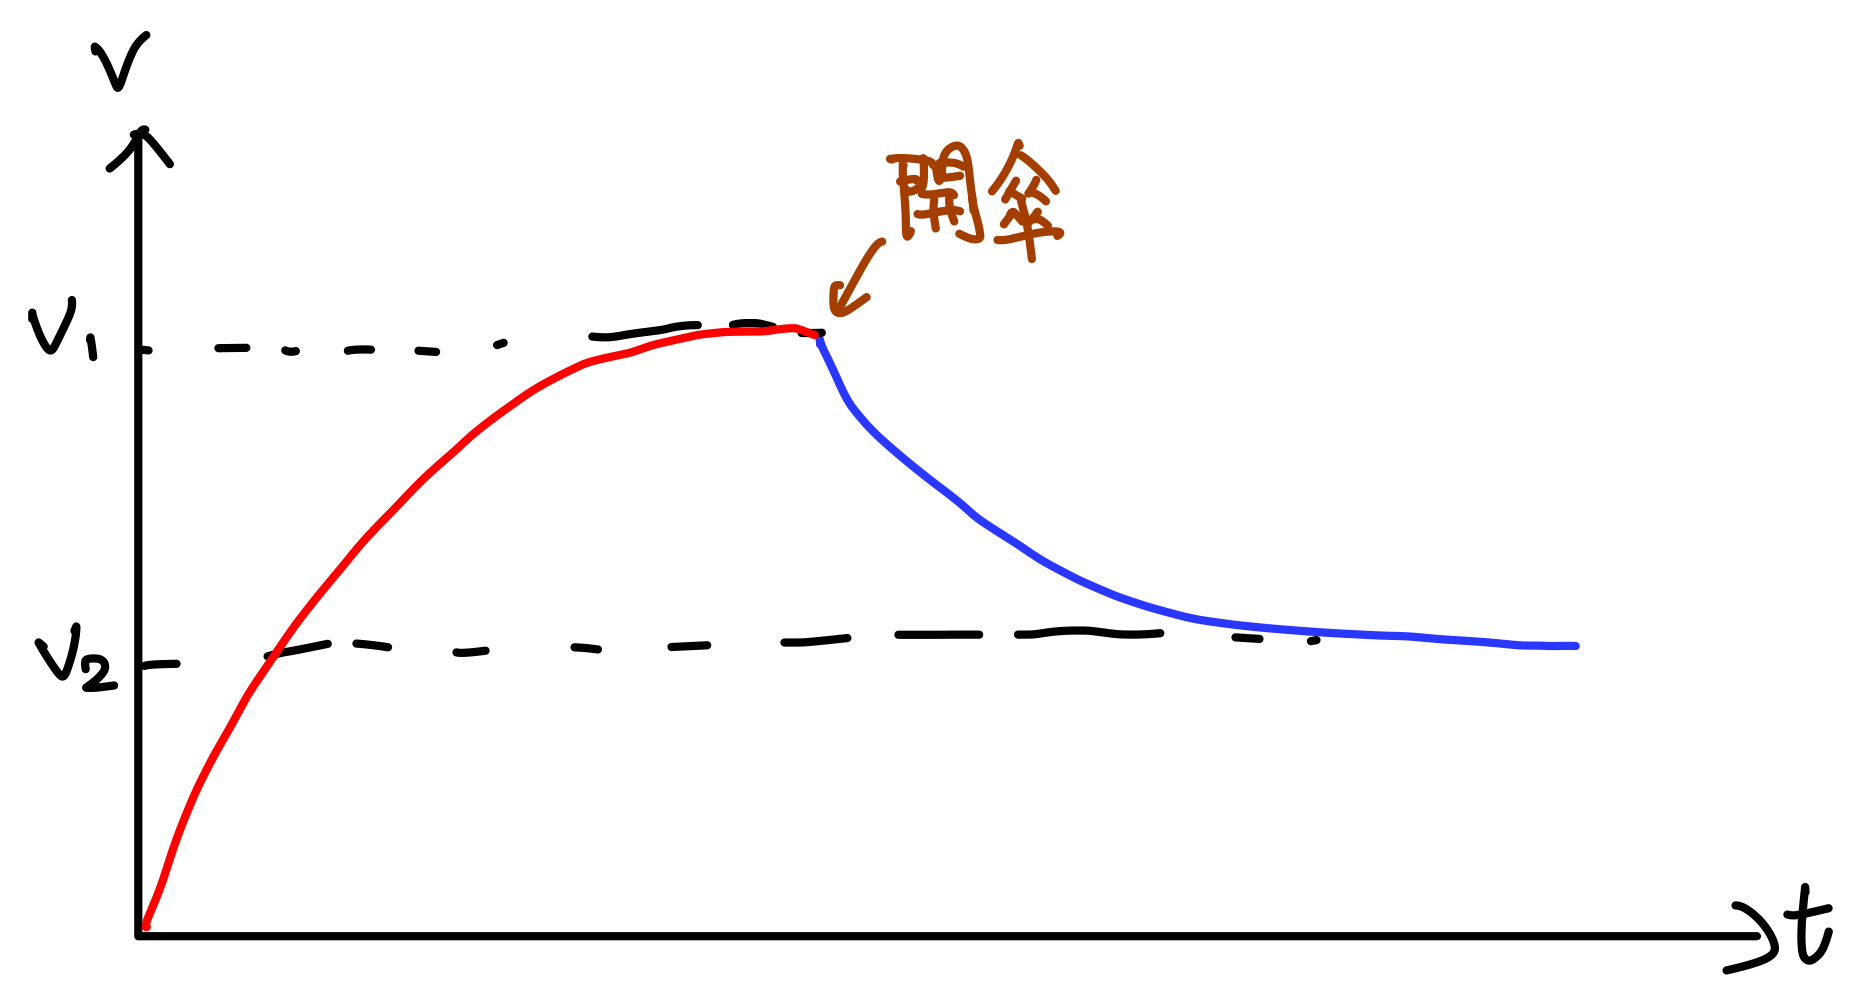
\includegraphics[width=.8\textwidth]{assets/7930445f.png}
        \caption{跳傘員的v-t線圖}
    \end{figure}
\end{frame}
\begin{frame}{For interested students...}
    \begin{figure}[h!]
        \centering
        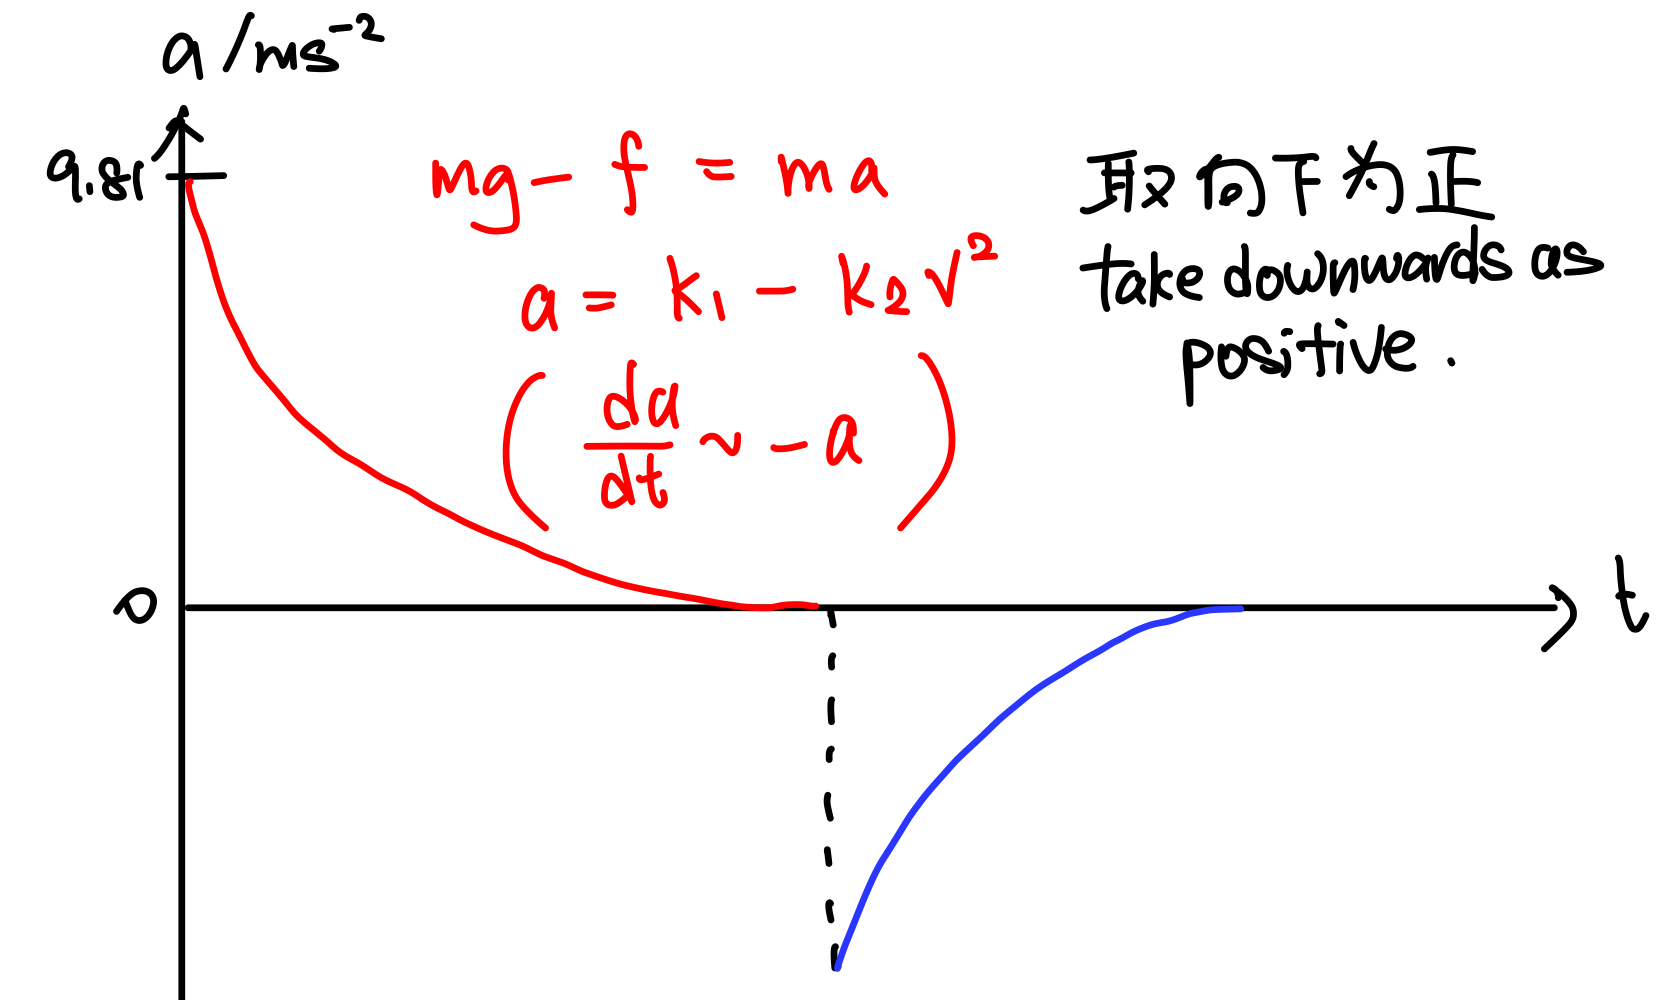
\includegraphics[width=0.55\textwidth]{assets/eda84940.png}
    \end{figure}
    \begin{figure}[h!]
        \centering
        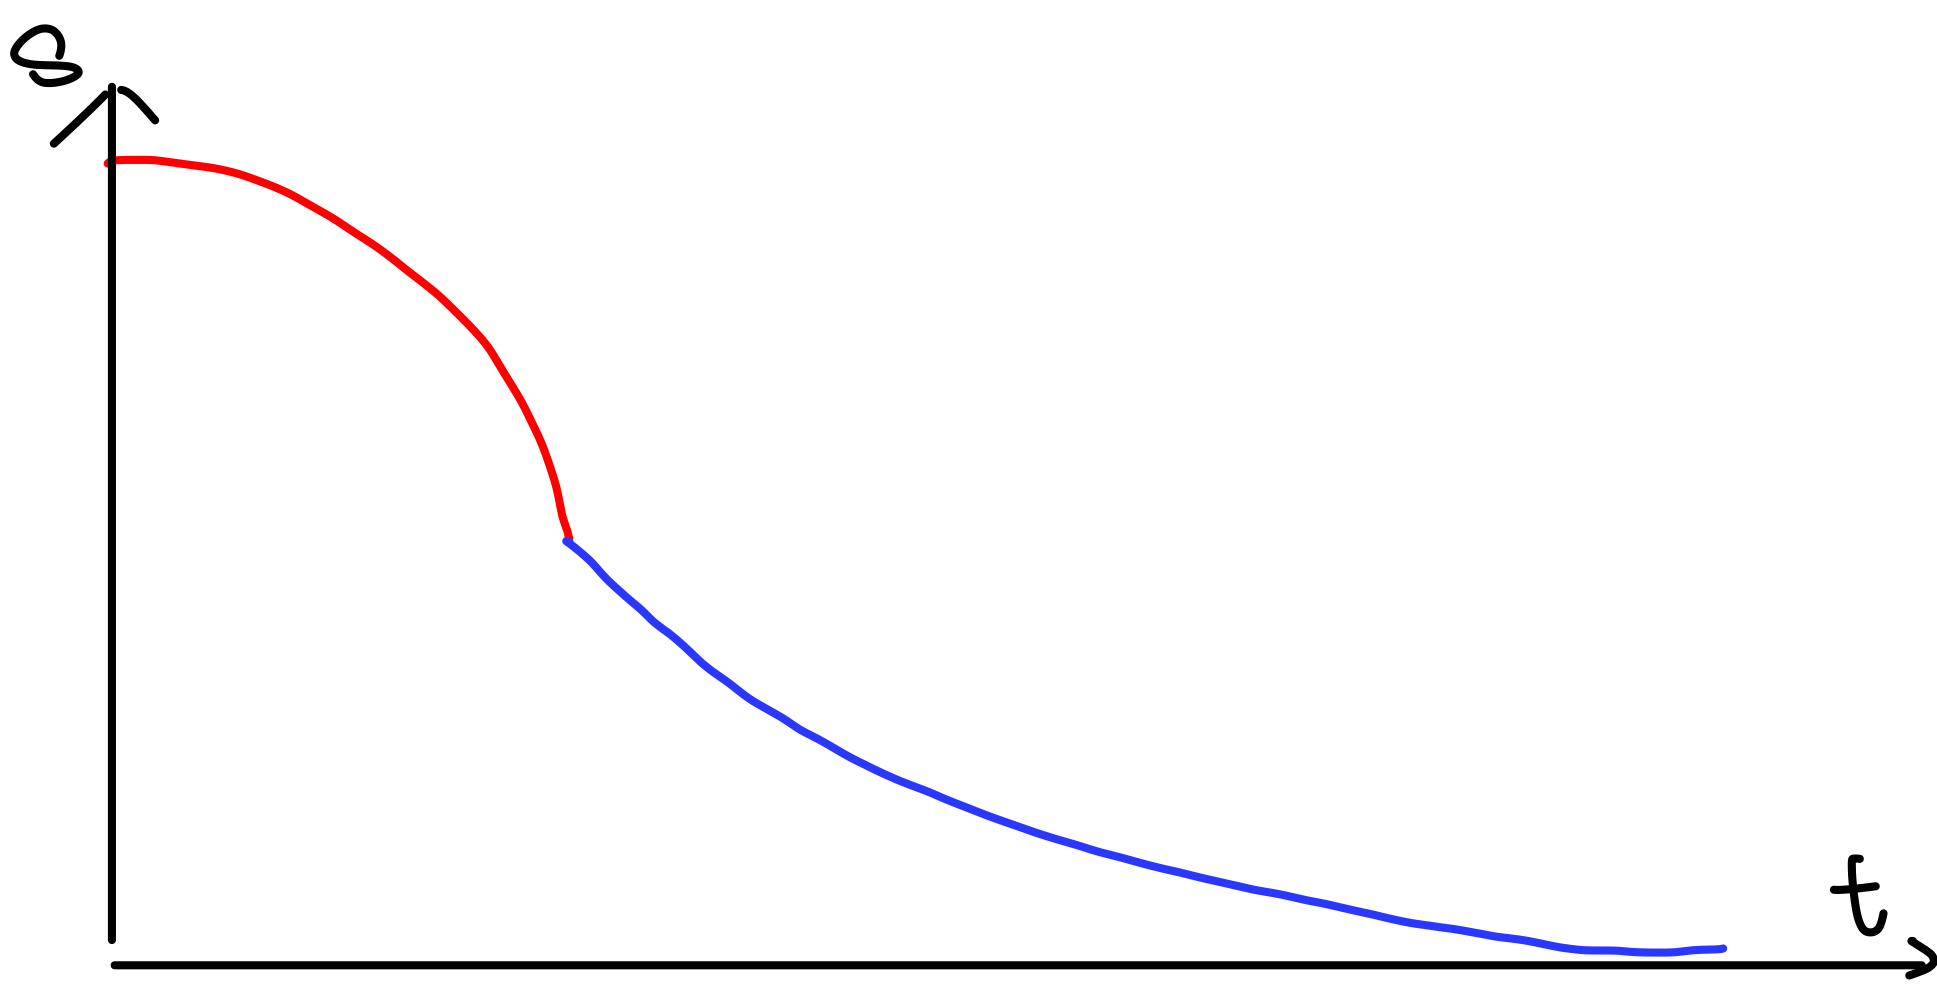
\includegraphics[width=0.55\textwidth]{assets/6689e5f4.png}
    \end{figure}
\end{frame}

\begin{frame}{牛頓第三定律 }
    \begin{exampleblock}
        {牛頓第三定律 }
        力總是成對出現。這些成對的力稱為作用力–反作用力對。
    \end{exampleblock}\bigskip
    \begin{figure}[h!]
        \centering
        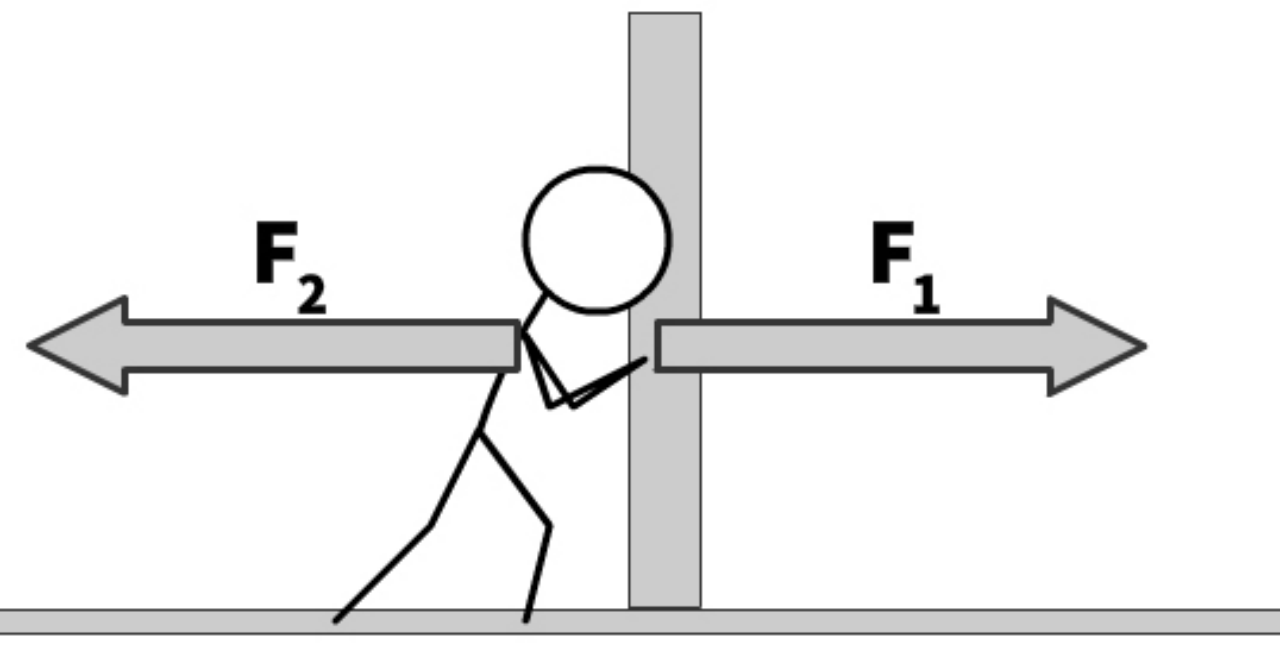
\includegraphics[width=.5\textwidth]{assets/350b642d.png}
    \end{figure}
\end{frame}
\begin{frame}{牛頓第三定律 }
    \begin{itemize}
        \item 作用力和反作用力的特性:
              \begin{itemize}
                  \item 量值相同
                  \item 方向相反
                  \item 作用於不同的物體
                  \item 必須屬於同一種力
              \end{itemize}
    \end{itemize}
\end{frame}
\begin{frame}{牛頓第三定律 }
    重量:
    \begin{figure}[h!]
        \centering
        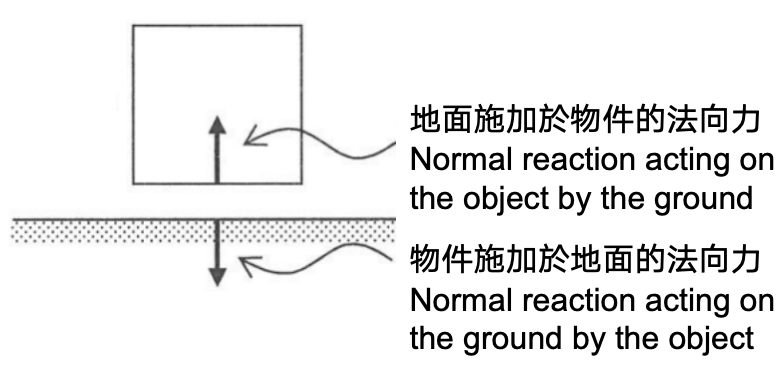
\includegraphics[width=.8\textwidth]{assets/4949a09b.png}
    \end{figure}
\end{frame}
\begin{frame}{牛頓第三定律 }
    法向力:
    \begin{figure}[h!]
        \centering
        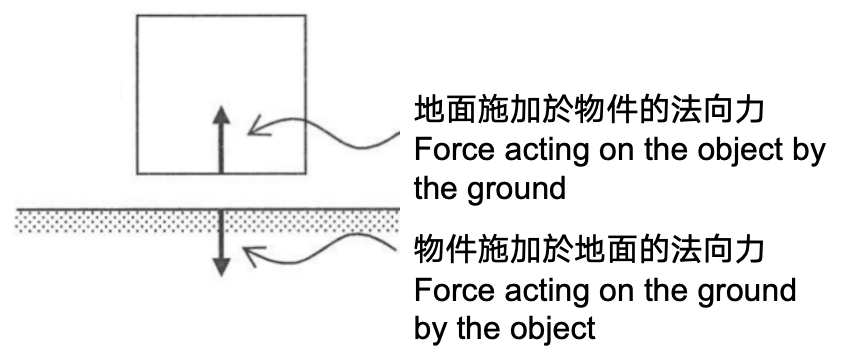
\includegraphics[width=.8\textwidth]{assets/69c3d3bd.png}
    \end{figure}
\end{frame}
\begin{frame}{牛頓第三定律 }
    張力:
    \begin{figure}[h!]
        \centering
        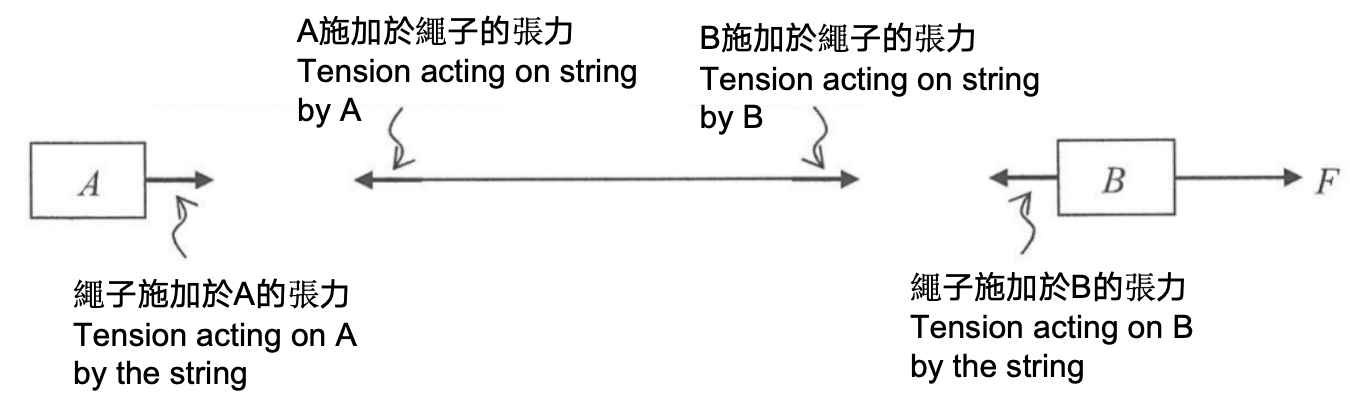
\includegraphics[width=.8\textwidth]{assets/f559bb67.png}
    \end{figure}
\end{frame}


\begin{frame}{牛頓第三定律 }
    \begin{figure}[h!]
        \centering
        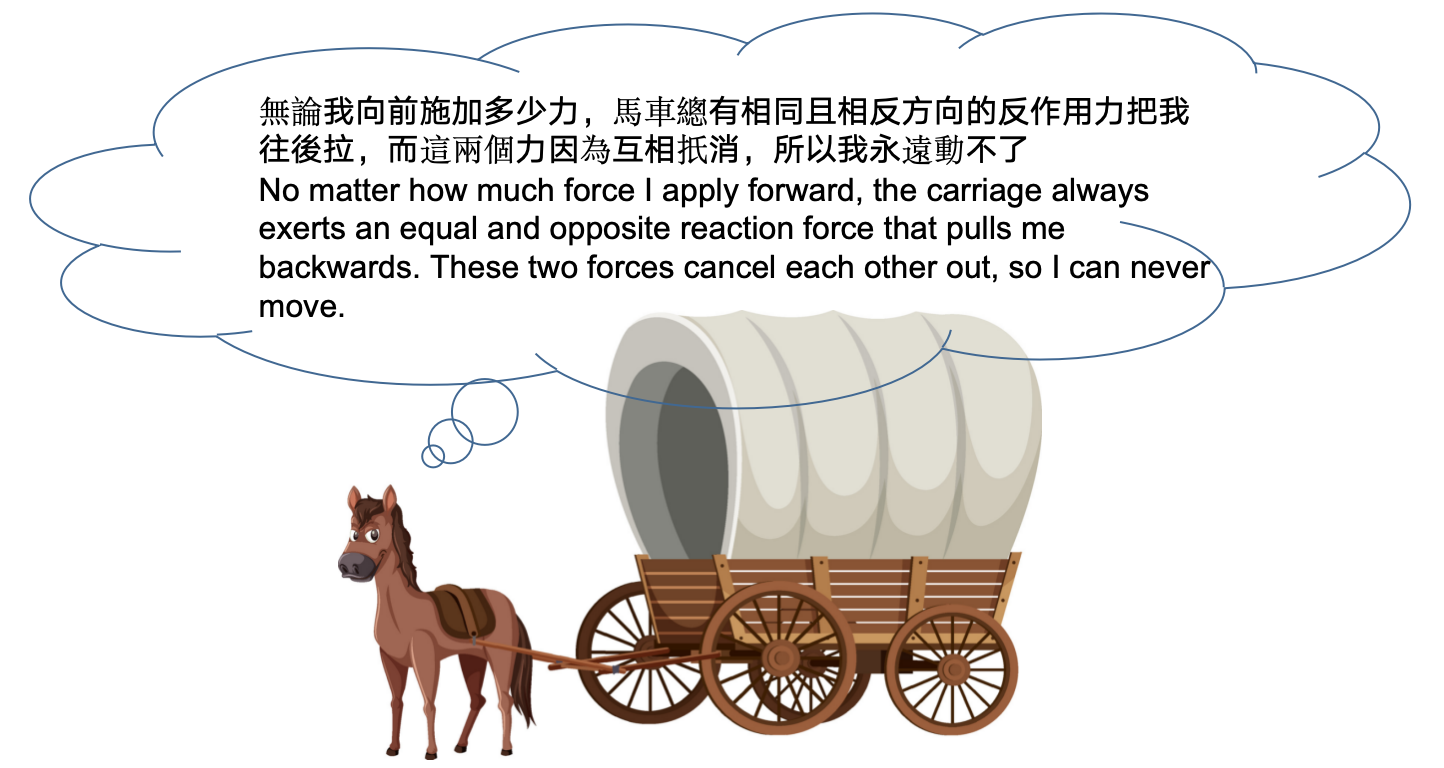
\includegraphics[width=\textwidth]{assets/4b5ef98a.png}
    \end{figure}
\end{frame}
\begin{frame}{牛頓第三定律 }
    \begin{figure}[h!]
        \centering
        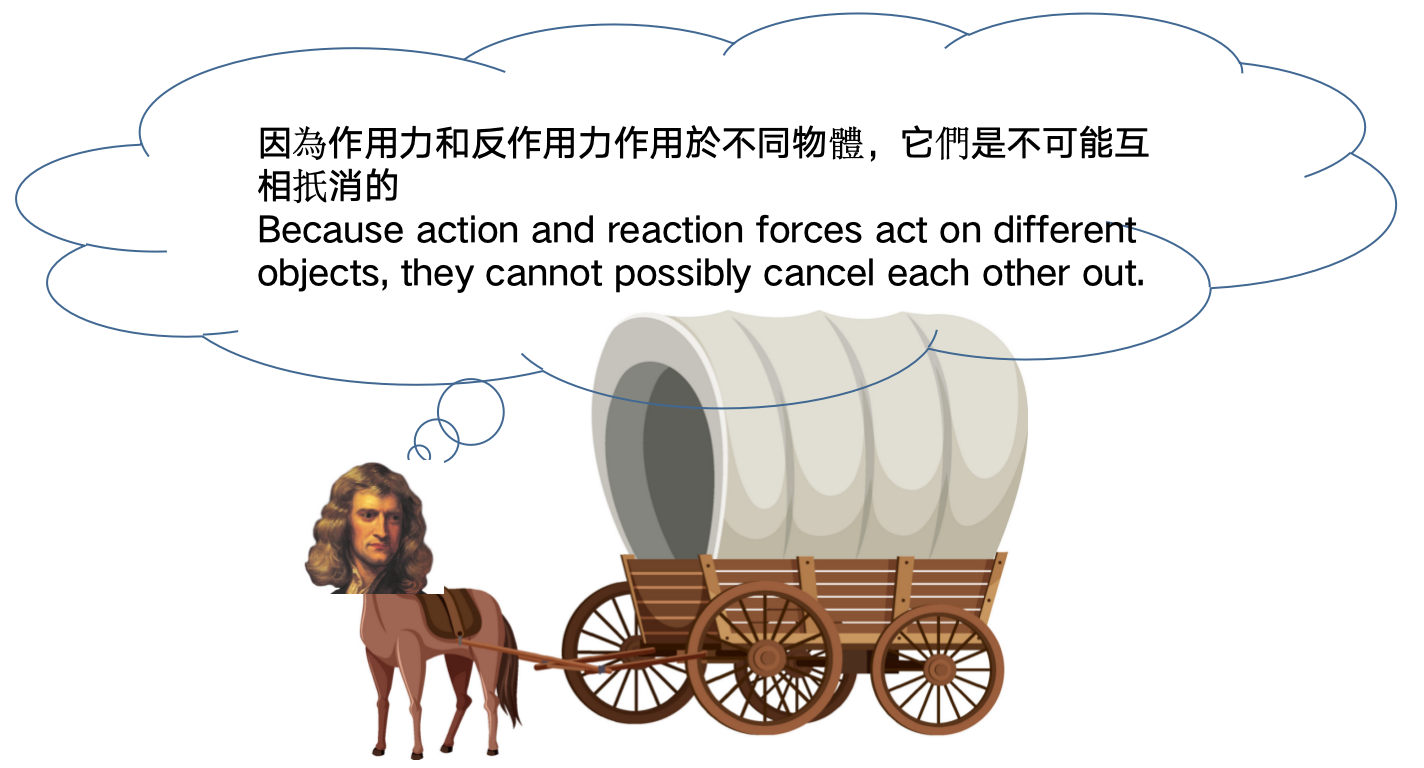
\includegraphics[width=\textwidth]{assets/9334d132.png}
    \end{figure}
\end{frame}

\begin{frame}{}
    \begin{figure}[h!]
        \centering
        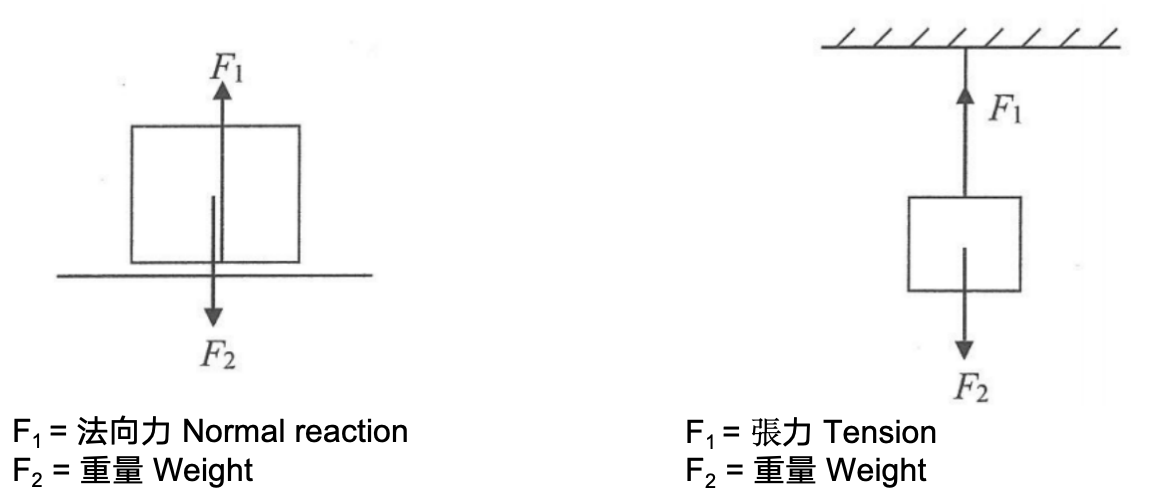
\includegraphics[width=.8\textwidth]{assets/6a71f82b.png}
    \end{figure}
    \begin{itemize}
        \item F$_1$ 和 F$_2$ 不是作用力反作用力對的理由:
              \begin{itemize}
                  \item 作用於相同物體
                  \item 屬於不同種力
              \end{itemize}
    \end{itemize}
\end{frame}



\begin{eg}
    \begin{figure}[h!]
        \centering
        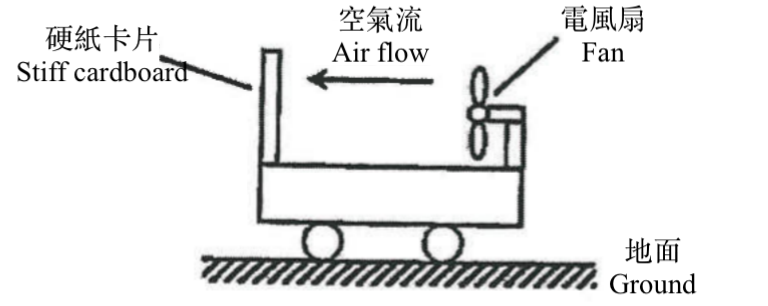
\includegraphics[width=0.66\textwidth]{assets/323c58f6.png}
    \end{figure}
    在小車的一端裝了電風扇,一張硬紙卡片固定在另一端且面向電風扇。當電風扇啓動後,小車將會怎樣運動?\\(a)不動(b)向左走(c)向右走(d)在原地往返運動


\end{eg}

\begin{eg}
    \begin{figure}[h!]
        \centering
        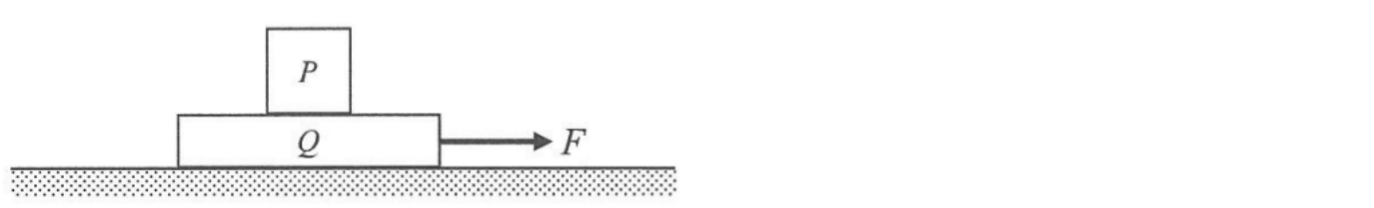
\includegraphics[width=.8\textwidth]{assets/9c913c73.png}
    \end{figure}
    P是 2kg,Q是 3kg,F 是 6N,所有接觸面都是光滑的。求P、Q的加速度。
\end{eg}

\begin{eg}
    \begin{figure}[h!]
        \centering
        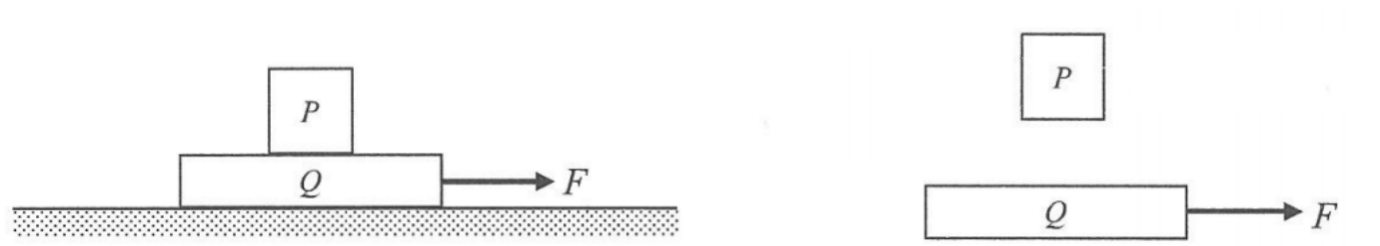
\includegraphics[width=.8\textwidth]{assets/5c3215d2.png}
    \end{figure}
    P是2kg,Q是3kg,F是6N,現在地面仍是光滑的,但P和Q之間存在摩擦力,使得P和Q能同時移動。求摩擦力的量值。
\end{eg}

\begin{frame}{作用力和反作用力的日常應用}
    \begin{figure}[h!]
        \centering
        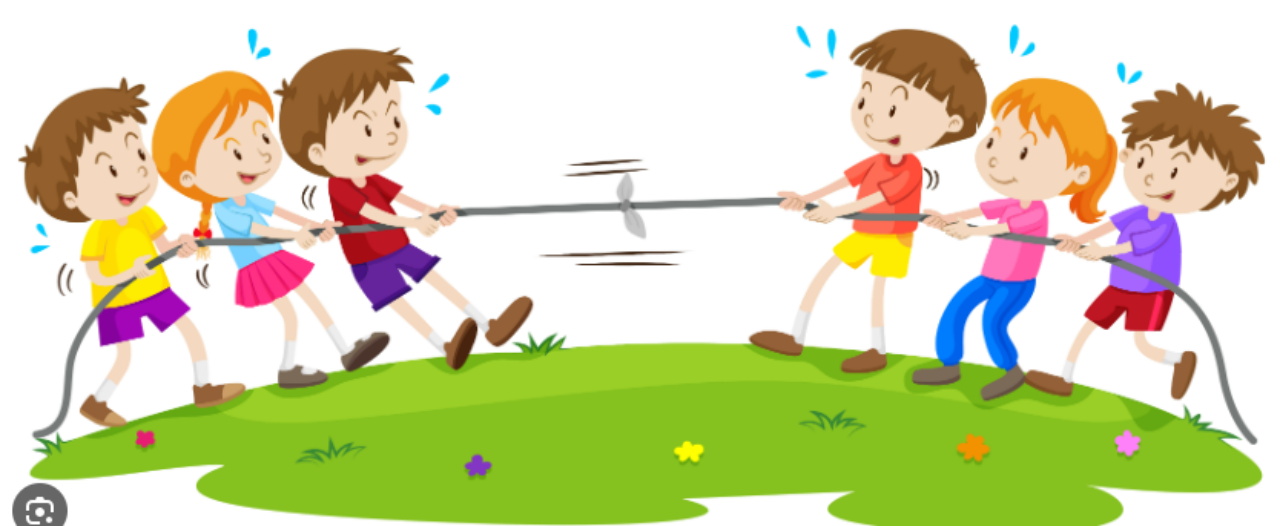
\includegraphics[width=.8\textwidth]{assets/ae0d3530.png}
    \end{figure}
    \begin{itemize}\bigskip
        \item 與地面產生的摩擦力大者勝出。
    \end{itemize}
\end{frame}
\begin{frame}{作用力和反作用力的日常應用}
    \begin{figure}[h!]
        \centering
        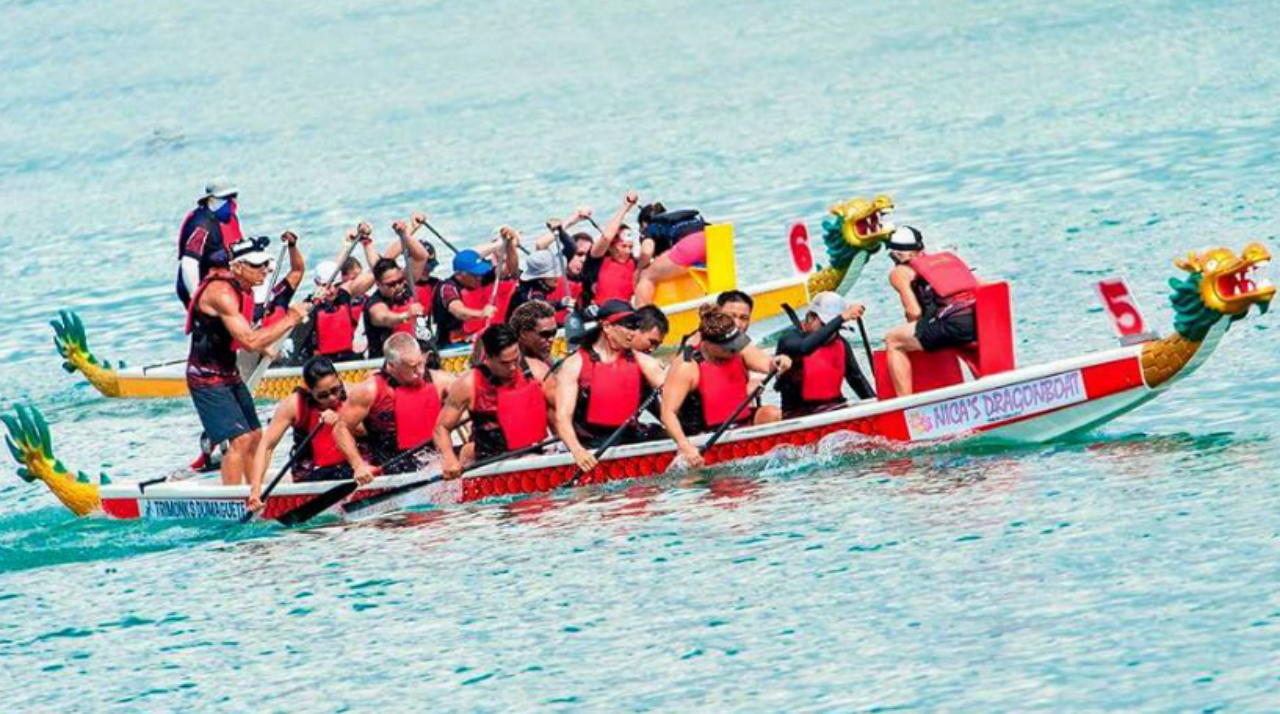
\includegraphics[width=.75\textwidth]{assets/45e1912d.png}
    \end{figure}
    \begin{itemize}
        \item 船槳向後推動河水,河水對船槳施加反作用力使船前進。
    \end{itemize}
\end{frame}
\begin{frame}{作用力和反作用力的日常應用}
    \begin{figure}[h!]
        \centering
        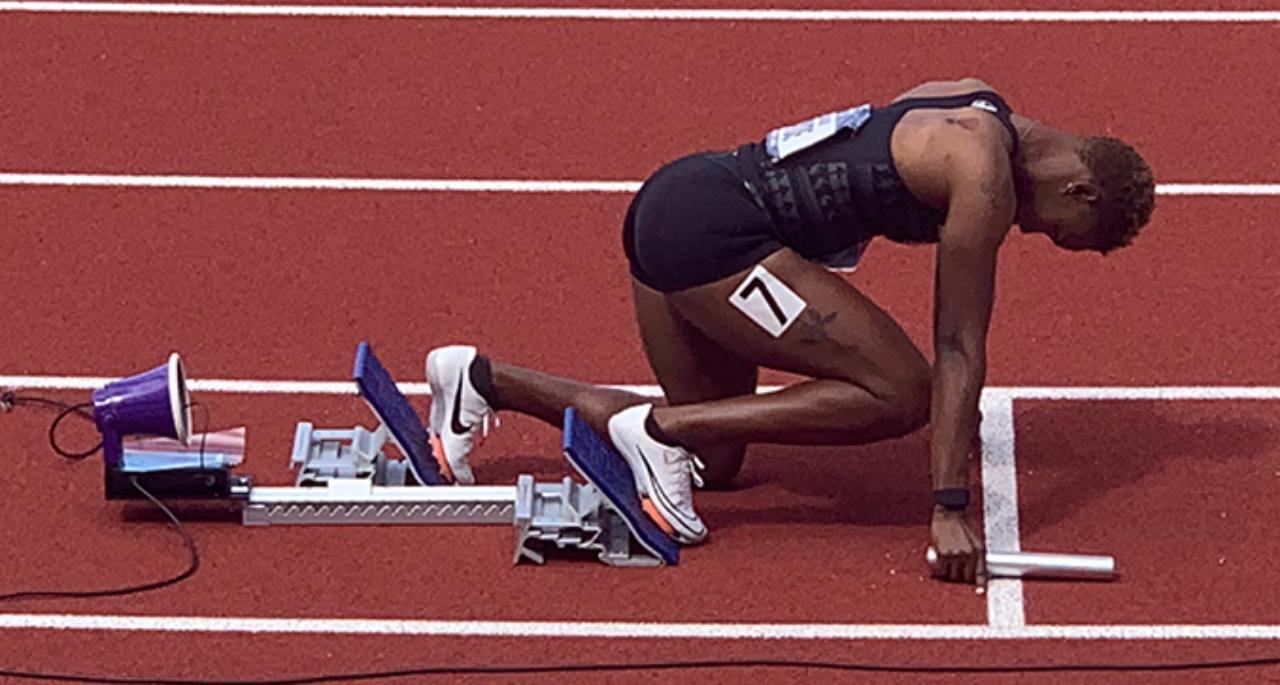
\includegraphics[width=.8\textwidth]{assets/60a0e41a.png}
    \end{figure}
    \begin{itemize}
        \item 助跑器為運動員在比賽開始時提供穩定且有爆發力的推動。
    \end{itemize}
\end{frame}
\end{document}